\documentclass[reprint,english,notitlepage]{revtex4-2}
\usepackage{amsmath}
\usepackage[mathletters]{ucs}
\usepackage[utf8x]{inputenc}
\usepackage[english]{babel}
\usepackage{esint}
\usepackage{physics,amssymb}
\usepackage{graphicx}
\usepackage{xcolor}
\usepackage{hyperref}
\usepackage{listings}
\usepackage{subfigure}
% \usepackage[style=science, backend=biber]{biblatex}
% \addbibresource{References_Part_4.bib} TODO: Slett før innlevering
\hypersetup{
    colorlinks,
    linkcolor={red!50!black},
    citecolor={blue!50!black},
    urlcolor={blue!80!black}}

\lstset{inputpath=,
    backgroundcolor=\color{white!88!black},
    basicstyle={\ttfamily\scriptsize},
    commentstyle=\color{magenta},
    language=Python,
    morekeywords={True,False},
    tabsize=4,
    stringstyle=\color{green!55!black},
    frame=single,
    keywordstyle=\color{blue},
    showstringspaces=false,
    columns=fullflexible,
    keepspaces=true}

\begin{document}

\title{Preparing For The Landing}
\author{Oskar Idland \& Jannik Eschler}
\date{\today}
\affiliation{Institute of Theoretical Astrophysics, University of Oslo}

\begin{abstract}
    By using a Hohmann transfer orbit, the altitude of the spacecraft's orbit has been lowered from $7.5 \times 10^7$ meters to $1 \times 10^6$ meters above the surface.
    When analysing the atmosphere using temperature, doppler shift, variation and flux, no gases were consistent options.
    Since the measurement using flux is the most reliable, it leads to the conclusion that the atmosphere is $100\%$ O$_2$.
    Using the onboard camera, the planets surface has been imaged to determine the most suitable landing site at the spherical coordinates [$R = 3775.2$ km, $\theta = 3.0257^{\circ}$ rad, $\phi = -2.5813^{\circ}$ rad].
\end{abstract}

\maketitle
\onecolumngrid
\section{Information} \label{sec:info}
\center{In this paper we would like to only be graded based on the programming, results and discussion.}

\section{Results} \label{sec: results}

\subsection{Spectral Analysis of the Atmosphere} \label{ssec: Analysis results}
\begin{table}[h!] \label{tab: Spec anal}
  \begin{tabular}{|c|*{4}{c|}}    
    \hline
    Gas  &Wavelength (nm) &Min. Flux &Temperature (K) &Doppler Shift (nm) \\
    \hline
    $ O_{2} $ &632 &0.90 &150.0 &8.96e-03 \\
    \hline
    $ O_{2} $ &690 &0.87 &450.0 &1.24e-02 \\
    \hline
    $ O_{2} $ &760 &0.93 &450.0 &1.58e-02 \\
    \hline
    $ H_{2}O $ &720 &0.95 &150.0 &2.27e-02 \\
    \hline
    $ H_{2}O $ &820 &0.91 &189.2 &1.48e-02 \\
    \hline
    $ H_{2} O$ &940 &0.87 &424.4 &7.55e-03 \\
    \hline
    $ CO_{2} $ &1400 &0.90 &450.0 &2.70e-02 \\
    \hline
    $ CO_{2} $ &1600 &0.93 &250.0 &5.56e-02 \\
    \hline
    $ CH_{4} $ &1660 &0.90 &150.0 &6.57e-03 \\
    \hline
    $ CH_{4} $ &2200 &0.90 &450.0 &4.36e-02 \\
    \hline
    $ CO $ &2340 &0.97 &216.7 &2.74e-02 \\
    \hline
    $ N_{2}O $ &2870 &0.97 &183.3 &3.32e-02 \\
    \hline
    \end{tabular}
  \end{table}
  \newpage
\twocolumngrid
% Figure~\ref{fig: O2 632},~\ref{fig: O2 690},~\ref{fig: O2 760},~\ref{fig: H2 720},~\ref{fig: H2 820},~\ref{fig: H2 940},~\ref{fig: CO2 1400},~\ref{fig: CO2 1600},~\ref{fig: CH4 1660},~\ref{fig: CH4 2200},~\ref{fig: CO 2340} \&~\ref{fig: N20 2870}
Depicted in the figures in section~\ref{subsec:figures-atmospheric-analysis} are the Gaussian line profile of possible gases contained in the target planets atmosphere.
Table~\ref{tab: Spec anal} depicts much of the same information in addition to the temperature.

On top of the plots we have added the noise from our data.
The noise have values in the range of 0.05 to 0.15, but for the sake of visualization we have added 0.95 as to lay the noise on top of the other data to make it easier to see its effect.

\subsection{Model of Planet Atmosphere}
\begin{figure}[h!]
  \centering
  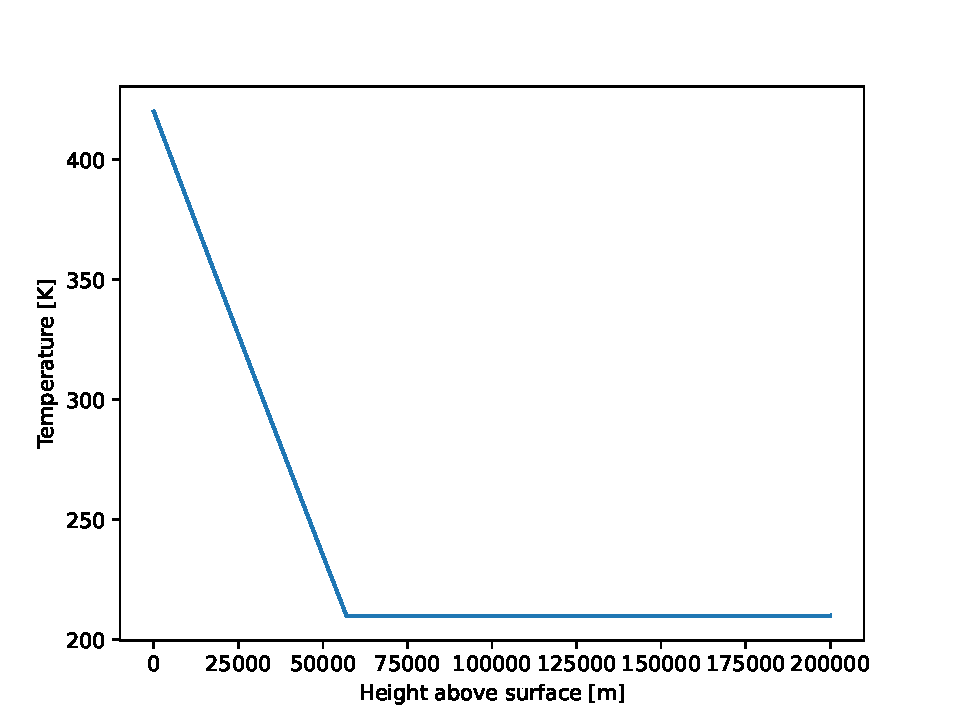
\includegraphics[scale = .4]{Figures/Temperature plot}
  \caption{Our model of the temperature as a function of meters above the surface }
  \label{fig: Temperature}
\end{figure}

\begin{figure}[h!]
  \centering
  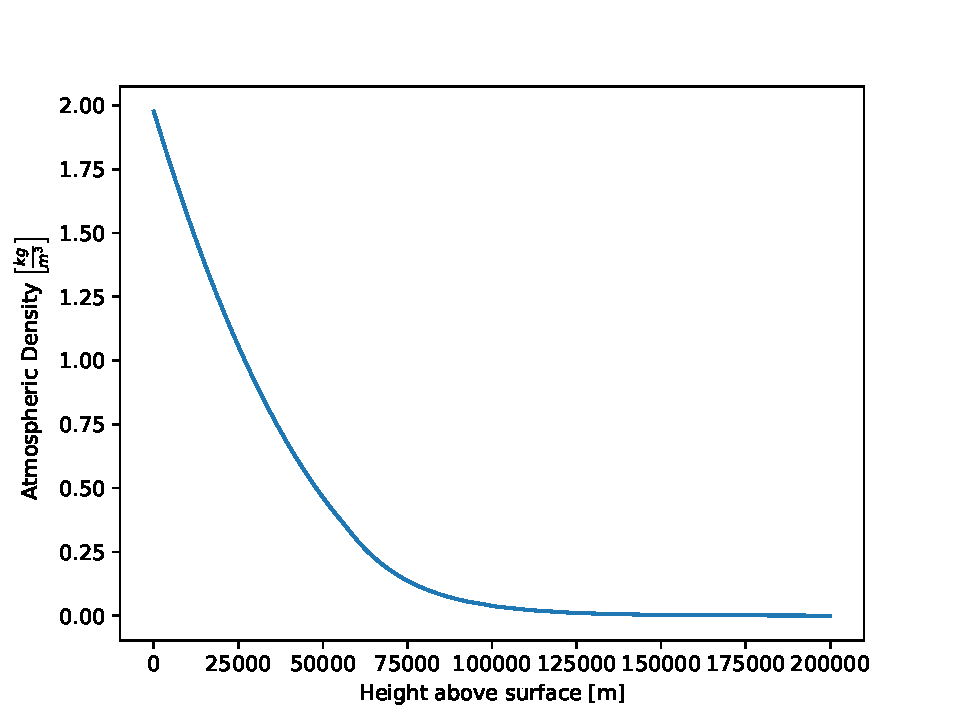
\includegraphics[scale = .4]{Figures/Density plot}
  \caption{Our model of the atmospheric density as a function of meters above the surface }
  \label{fig: Density}
\end{figure}


\subsection{Lowering the orbit}\label{subsec:lowering-the-orbit}
    After completing the journey to Planet 1 and entering a high altitude orbit around the planet, we now used a Hohmann transfer maneuver to decrease the orbital height to a low-altitude orbit.
    The initial orbital height was around 75'000 km above the surface of the planet.
    To get a better view of the planet, two controlled boosts were executed.
    The first one to enter an elliptical transfer orbit from the initial orbit introduced a speed of change of
    The change of speed during each burn have been calculated to be
    \begin{align*}
        &\Delta v_0 = -1190.3 \,\text{m/s}\\
        &\Delta v_1 = 519.76 \,\text{m/s}
    \end{align*}

    The calculations for these values can be found in section~\ref{subsec:calculation-of-the-hohmann-transfer-orbit}.\\

    After the Hohmann transfer orbit and both boosts have been executed, we entered a new orbit with an orbital altitude of $1 \times 10^6$ meters above the surface of the planet.\\

    To verify the stability of the orbit, we first measured the average height of the orbit.
    Thereafter, the spacecraft orbited the planet for $1 \times 10^6$ seconds, before measuring the average height again.
    This resulted in an altitude difference of $-64.92$ meters over the course of $12.73$ days.


\subsection{Finding landing sites}\label{subsec:finding-landing-sites}
    In our lower orbit we were now able to take more precise observations of the surface of the planet, and therefore scout for possible landing sites.
    Over the course of $15$ minutes, the spacecraft has therefore been taking 15 pictures in equally spaced intervals of $1$ minute, pointing straight towards the planet.\\
    As we can see in Figures in section~\ref{subsec:potential-landing-sites}, the planets surface consists of both oceans, which are a dark green-blue colour and have an even texture.
    In the oceans, there are some islands, which are a dark green colour and partially have high mountains.\\
    The view of some islands and oceans are obstructed by the blue-coloured clouds, but by using information of multiple images, we can see that there is a large island right underneath in Figure~\ref{fig:l_site6} and~\ref{fig:l_site7}.\\

    The spherical coordinates of each of the imaged landing sites in section~\ref{subsec:potential-landing-sites} can be seen in table~\ref{tab:land_coords}.
    Radius stands for the distance of the positions to the center of the planet, theta is the angle between the z-axis and the line from the center of the planet and the spacecraft, and phi is the angle between the x-axis and the line between the center of the planet and the spacecraft.
    All coordinates are relative to the position of the planet at the time when we entered the lower-altitude orbit.\\
    \begin{table}[h]
        \begin{tabular}{|c|c|c|c|}
            %% l (Left aligned), c (Centered), r (Right aligned)
            \hline
            Site Nr. & Radius [km] & $\,\theta$ [rad] & $\,\phi$ [rad]\\
            \hline
            Site 0 & 3775.2 & 3.0479 & -2.8217\\
            \hline
            Site 1 & 3775.2 & 3.0442 & -2.7816\\
            \hline
            Site 2 & 3775.2 & 3.0405 & -2.7415\\
            \hline
            Site 3 & 3775.2 & 3.0368 & -2.7015\\
            \hline
            Site 4 & 3775.2 & 3.0331 & -2.6614\\
            \hline
            Site 5 & 3775.2 & 3.0294 & -2.6213\\
            \hline
            Site 6 & 3775.2 & 3.0257 & -2.5813\\
            \hline
            Site 7 & 3775.2 & 3.0220 & -2.5412\\
            \hline
            Site 8 & 3775.2 & 3.0183 & -2.5011\\
            \hline
            Site 9 & 3775.2 & 3.0146 & -2.4610\\
            \hline
            Site 10 & 3775.2 & 3.0109 & -2.4210\\
            \hline
            Site 11 & 3775.2 & 3.0072 & -2.3809\\
            \hline
            Site 12 & 3775.2 & 3.0035 & -2.3408\\
            \hline
            Site 13 & 3775.2 & 2.9998 & -2.3008\\
            \hline
            Site 14 & 3775.2 & 2.9961 & -2.2607\\
            \hline
        \end{tabular}
        \caption{Spherical coordinates of the potential landing sites imaged in section~\ref{subsec:potential-landing-sites}}
        \label{tab:land_coords}
    \end{table}

    As it is preferable to land on land, the island in landing site 6 offers a well suited landing site for our purposes.
    By landing on land, we will also be able to take probes of the soil on planet 1, to determine it's composition.

\section{Discussion} \label{sec: discussion}
\subsection{Spectral Line Analysis} \label{ssec: Spec Anal}
  
To filter out spectral lines which were flukes we used a multitude of criteria.

\begin{itemize}
  \item Temperature of different spectral lines in one gas
  \item Variation in the analysis with different levels of accuracy
  \item Doppler shift
  \item Amount of flux
  \item How good a fit the calculated line is in comparison to measurements
\end{itemize}

Of a real spectral line we expect the lines to have about the same temperature. This was not the case for either $ O_{2} $, $ H_2O  $, $ CO_2 $ and $ CH_4 $. We therefore doubt them being possible gases in the atmosphere.
\newline

When running our analysis we could choose whatever accuracy we wanted. As our accuracy got higher a lot of our results changed temperature drastically. This was to our advantage as it most likely meant the spectral line was a fluke. Using this as a criteria we can could be even more secure in our choice to doubt $ O_2 $, $ H_2O $ and $ CH_4 $. The temperature of $ CO $ and $ N_2O $  converged towards 217 K and 183 K respectivly as seen in table \ref{tab: Spec anal}.
\newline

The Doppler shift is quite inconsistent in most cases. We clearly observe this in $ CO_2 $, $ H_2O $ and $ CH_4 $ in which we observe the absolute shift being around 2 times as much for $ CO_2 $, 2-3 times as much for $ H_2O $ and 7 times as much for $ CH_4 $. In all other cases their are either just one line per gas or consistent results. $ O_2 $ had very consistent results. 
\newline

The flux was on the higher end of what we expected (0.7 $ \rightarrow  $ 1). Only a single line of $ O_2 $ and $ H_2O $ broke through 0.90. We expect to see a lower flux for real spectral lines. The most likely candidates so far being $ N_2O $ and $ CO  $ both had a very high flux of 0.97 which makes it more uncertain they are real.
\newline

When looking into which spectral lines fit the measured data the most we also need to take the noise into account. The more noise, the higher the likelihood of fluctuations looking like spectral lines. We will focus on the parts of the graphs where the noise is relatively low and seemingly bounces of the Gaussian line distribution. 
\subsubsection*{$ O_2 $}
The first spectral line of $O_2$ at 632 nm \ref{fig: O2 632} is not too far off the peak of the noise and has a big fluctuations all around. This seems to most likely be a fluke. 

The second spectral line of $O_2$ at 690 nm \ref{fig: O2 690} is very close to a local minima point. Comparing this to every other local minima of the noise we see our line profile gives a good match with the lowest fluctuations of all the local minimums. This seems to be a real line 

The third spectral line of $O_2$ at 760 nm \ref{fig: O2 760} is also very close to a local minima and our line profile seems like a good fit here as well. Out of all the local minima points this also seems like the most likely to contain a true line. 

Just looking at the graphs we observe oxygen giving us two seemingly good fits.  

\subsubsection*{$ H_2O $}
All the line profiles of $ H_2O $ seen in \ref{fig: H2 720}, \ref{fig: H2 820} and \ref{fig: H2 940} Are surrounded by a lot of data not matching our line profile, and do not seem like good fits. 

\subsubsection*{$ CO_2 $}
The first spectral line of $ CO_2 $ seen in \ref{fig: CO2 1400} is close to a local maxima of noise so we can not say with certainty wether or not this is a true line or just a fluke. 

The second spectral line of $ CO_2 $ seen in \ref{fig: CO2 1600} is located very close to a local minima of noise which gives us confidence in its validity, but our curve is not the best fit for the measured data. 

When taking both graphs into account it seems likely that none of the spectral lines of $ CO_2 $ are real. 

\subsubsection*{$ CH_4 $}
The first spectral line of $ CH_4 $ seen in \ref{fig: CH4 1660} is not too far off a local minima of noise, but there are a lot of measured flux above our line profile, which may point to it not being a real line after all. Our graph does not fit the measured data very well either. 

The second spectral line of $ CH_4 $ seen in \ref{fig: CH4 2200} is located in between a local minima and maxima and follows the measured data quite nicely. Its the only local minima with a dip in flux over a wide range. This might be a sign the line is real. 

Judging by its graphs its very hard to say weather or not the graphs actually represent real lines. 

\subsubsection*{$ CO $}
The spectral line of $ CO $ seen in \ref{fig: CO 2340} is surrounded by a bit different data. In this case, the noise was relatively small in comparison with the measured data. This means the noise will have less an effect on the flux. When the flux varies this much with such small amounts of noise its not very likely this is a real line. Our line profile does not match too well with the measured data either. 

\subsubsection*{$ N_2O $}
The spectral line of $ N_2O $ seen in \ref{fig: N20 2870} is located right under a local maxima which makes it more likely the measured dip in flux is a result of chance and noisy data. Looking at the rest of the graph there seems to be no dip of significance around any of the local minima. 


\subsection{Lowering the orbit}\label{subsec:lowering-the-orbit-disc}
    The Hohmann transfer is a difficult maneuver to execute.
    The boosts need to be executed at exactly the right time and exactly deliver the calculated impulse to the spacecraft.
    However, since our team consists of some of the best scientists of our country, we were able to execute the boosts as planned.
    Furthermore, it is possible to do some correction burns in case the main boosts into the Hohmann transfer orbit and into the lower, circular orbit did not work exactly as expected.\\
    The solar winds from the star in our solar system are negligible when we are so close to the planet.
    But we will have to account for the gravitational forces from the small objects close to us.
    These can alter the trajectory of the spacecraft, which means we need to do some corrections to the trajectory to successfully execute the orbit transfer.
    In our simulations, we did not perform major corrections, but could have done if necessary, which means no significant unknown forces acted on the spacecraft during the transfer.\\

    When performing the orbit stability confirmation, we saw that the orbital height of the spacecraft was lowered by apporoximately $64$ meters.
    This corresponds to $0.0013$\% of the total orbital radius, which is not significant for a period of 12 days and 18 hours.\\
    The measurements are very reliable, as each of the orbital heights are based on the average of $1000$ measurements, taken at equally spaced positions around the entire orbit.\\

    One way to explain for the difference in orbital height is atmospheric drag.
    We are in a low-altitude orbit, which means that there will be a very thin atmosphere where we are.
    From figure~\ref{fig: Density} we can see that the density of the atmosphere converges to 0, but still has a clear non-zero value at our orbital height.
    This means, that the spacecraft constantly experiences some drag, which causes it to slow down very gently and therefore the orbital height to decrease.


\subsection{Finding landing sites}\label{subsec:finding-landing-sites-disc}
    The coordinates found for the landing sites were based on basic trigonometry, and assuming that the planet has a constant angular velocity around it's z-axis.
    Given the pictures we took, it is possible to identify a suitable landing site.
    The clouds do make it a bit more difficult, as they limit our view.
    However, as we have taken multiple picture, we could look at the landing site from multiple angles, which gave us a lot more information.\\

    Due to the specifications of our camera, we were not able to get a very close up view of a landing site.
    This will make things a bit more challenging when landing, but since we can make small adjustments when landing, it is sufficient to find a relatively clear area.
    The large island in figure~\ref{fig:l_site6} provides such an area with clearance in all directions, which allows for some deviance.\\

    All other landing sites either provide too little information due to the clouds, or are very close or on the ocean.
    They therefore provide only little, or no room for our landing, which makes them less suitable.



\section{Conclusion} \label{sec: conclusion}
\subsection{Atmosphere composition} \label{ssec: Atmpos Comp}
Judging by temperature, Doppler shift and variation in analysis it seems $ CO $ and $ N_2O $ is the only viable options.
These two have the most consistent and almost equal temperature.

Judging by the flux, $ CO $ and $ N_2O  $ are the worst option.
On the other hand, $ O_2 $ and $ CH_4 $ rises as the best options.

Judging by how good a fit our model is, we observe $ O_2 $ being the best fit by far. 

To conclude the discussion of results as seen in \ref{ssec: Spec Anal}, there is no clear candidate which checks all the boxes.
We choose to consider how well a fit our model is in addition to the flux the most important factors as that is based in actual data and not our just our own calculations.
The line profile seen in \ref{fig: O2 690} and \ref{fig: O2 760} matches a lot closer than the one seen in \ref{fig: O2 632}.
As the temperature of the first two are equal (450 $ K $) which also matches earlier estimates made in %~\parencite[][]{part3} TODO: Remove Comment
of the planets temperature, we will assume they are real lines.
The atmosphere is therefore 100 \% $ O_2 $ with a mean molecular weight $ \mu $ of
\[
\mu =   \frac{2 ⋅ 15.9994 ⋅  1.66 ⋅ 10^{-27}}{1.00794 ⋅ 1.66  ⋅  10^{-27}} = 31.75.
\]

\subsection{Finding landing sites from lower orbit}\label{subsec:finding-landing-sites-from-lower-orbit}
    By using a Hohmann transfer orbit, which included two main boosts of our spacecraft, we were able to successfully decrease the orbital altitude from $7.5 \times 10^7$ to $1 \times 10^{6}$ meters above the surface of the planet.
    The maneuver resulted in a relatively stable orbit around the planet.
    When measuring the altitude before and after a 12 day and 18 hour period, the altitude of the orbit decreased by only $64.92$ meters.
    The main reason for this decrease is due to atmospheric drag.
    Due to the low orbital height, we entered the top of the atmosphere, which has a very low density, but still exerts a slight, constant force on the spacecraft.
    This caused a decrease in speed, and therefore altitude.\\

    From the lower orbit we were able to scout for potential landing sites using the onboard camera.
    In figure ~\ref{fig:l_site6} we were able to see a relatively large island, which provides a large area in all directions and therefore is suitable for our purposes.
    The spherical coordinates of the preferred landing site are\\
    \begin{align*}
        \text{Radius}:&\; 3775.2 \;\text{km}\\
        \theta :&\; 3.0257^{\circ} \;\text{rad}\\
        \phi :&\; -2.5813^{\circ} \;\text{rad}
    \end{align*}

    These coordinates are relative to the position of the planet at the point in time when we entered the lower orbit.

\section{Appendix} \label{sec: appendix}
\subsection{Calculation of the Hohmann transfer orbit}\label{subsec:calculation-of-the-hohmann-transfer-orbit}
    The calculations of the boosts for the Hohmann transfer orbit are based on theory from %~\parencite[][]{hohmann_wiki}. TODO: Remove comment
    The magnitude of the boosts are calculated using the formulae for kinetic and potential energy.
    This results in the formulae for the boosts $\Delta v_0$ and $\Delta v_1$ being
    \begin{align*}
        \Delta v_0 = -\sqrt{\frac{\mu}{r_1}} \left(\sqrt{\frac{2r_0}{r_0 + r_1}}-1\right)\\
        \Delta v_1 = -\sqrt{\frac{\mu}{r_0}} \left(1-\sqrt{\frac{2r_1}{r_0 + r_1}}\right)
    \end{align*}
    Where $r_0$ is the radius of the initial, higher orbit, $r_1$ is the radius of the lower target orbit and $\mu$ is the standard gravitational parameter.

    The first boost was done at an arbitrary point in time, as the initial orbit was circular.
    However, the second boost had to be timed very well, which meant after $\frac{T}{4}$, where $T$ is the orbital period of the Hohmann transfer orbit.
    This way, the second boost will be executed at the perihelion of the transfer orbit and inject us in the desired orbit.


\onecolumngrid
\clearpage
\subsection{Figures from Atmospheric analysis}\label{subsec:figures-atmospheric-analysis}
    \begin{figure}[h!]
        \centering
        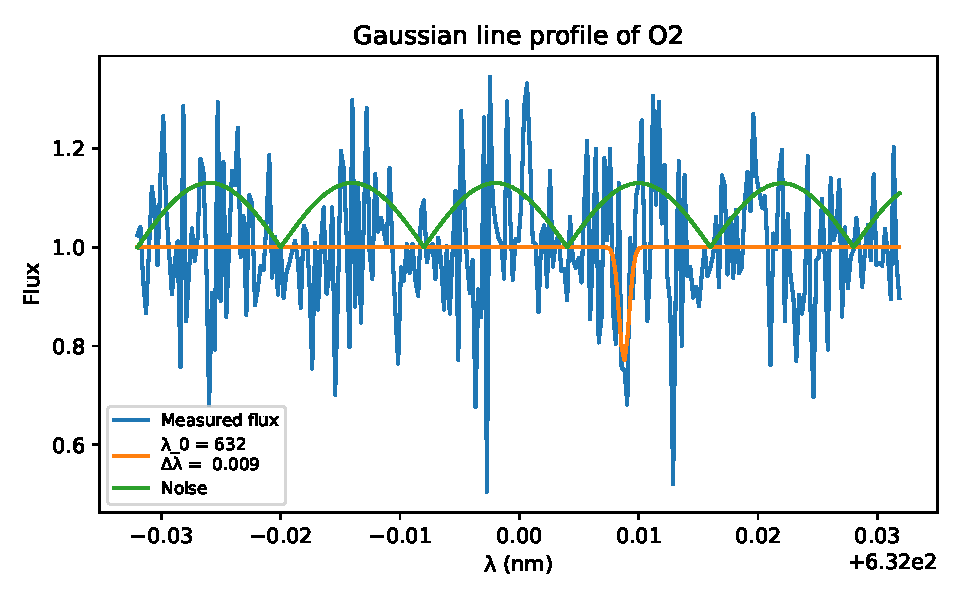
\includegraphics[scale =.3]{Figures/O2 632}
        \caption{Flux Data and Spectral Line Analysis}
        \label{fig: O2 632}
    \end{figure}

    \begin{figure}[h!]
        \centering
        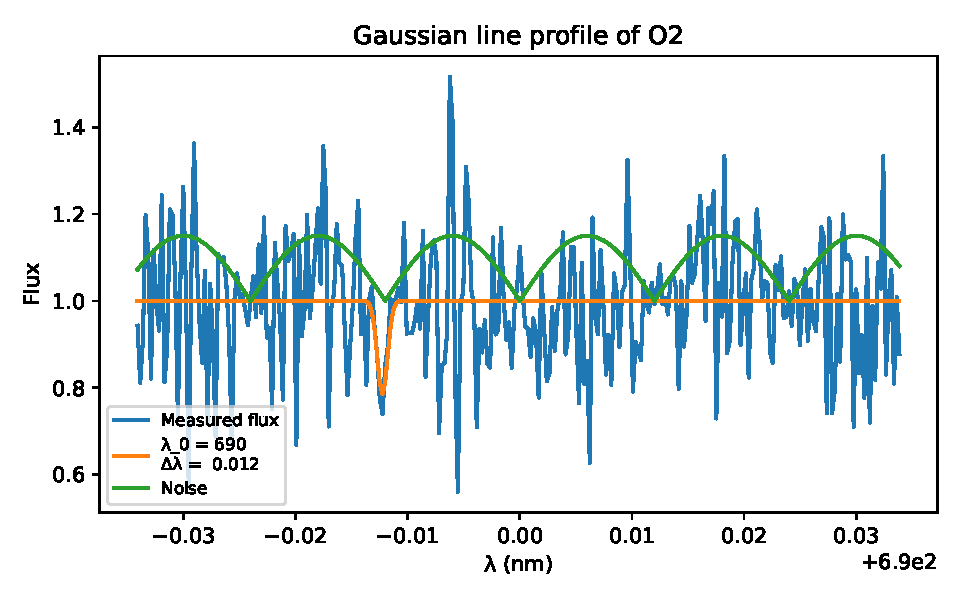
\includegraphics[scale =.3]{Figures/O2 690}
        \caption{Flux Data and Spectral Line Analysis}
        \label{fig: O2 690}
    \end{figure}

    \begin{figure}[h!]
      \centering
      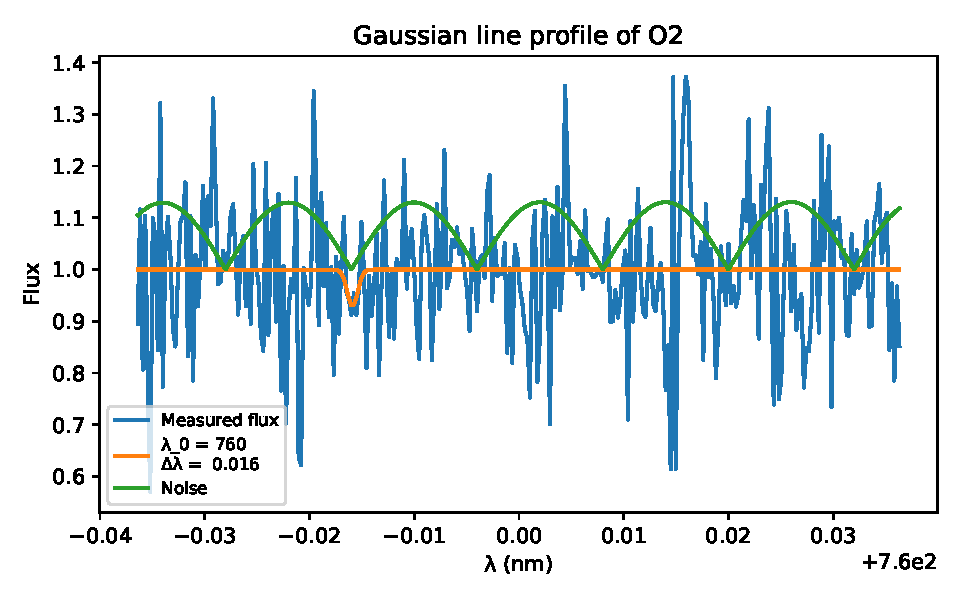
\includegraphics[scale =.3]{Figures/O2 760}
      \caption{Flux Data and Spectral Line Analysis}
      \label{fig: O2 760}
    \end{figure}

    \begin{figure}[h!]
      \centering
      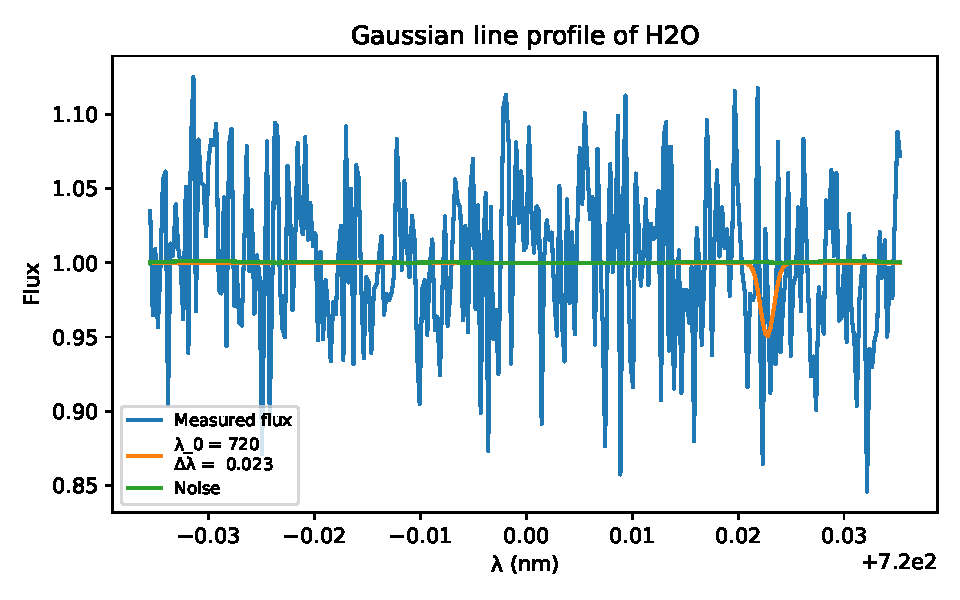
\includegraphics[scale =.3]{Figures/H2O 720}
      \caption{Flux Data and Spectral Line Analysis}
      \label{fig: H2 720}
    \end{figure}

    \begin{figure}[h!]
      \centering
      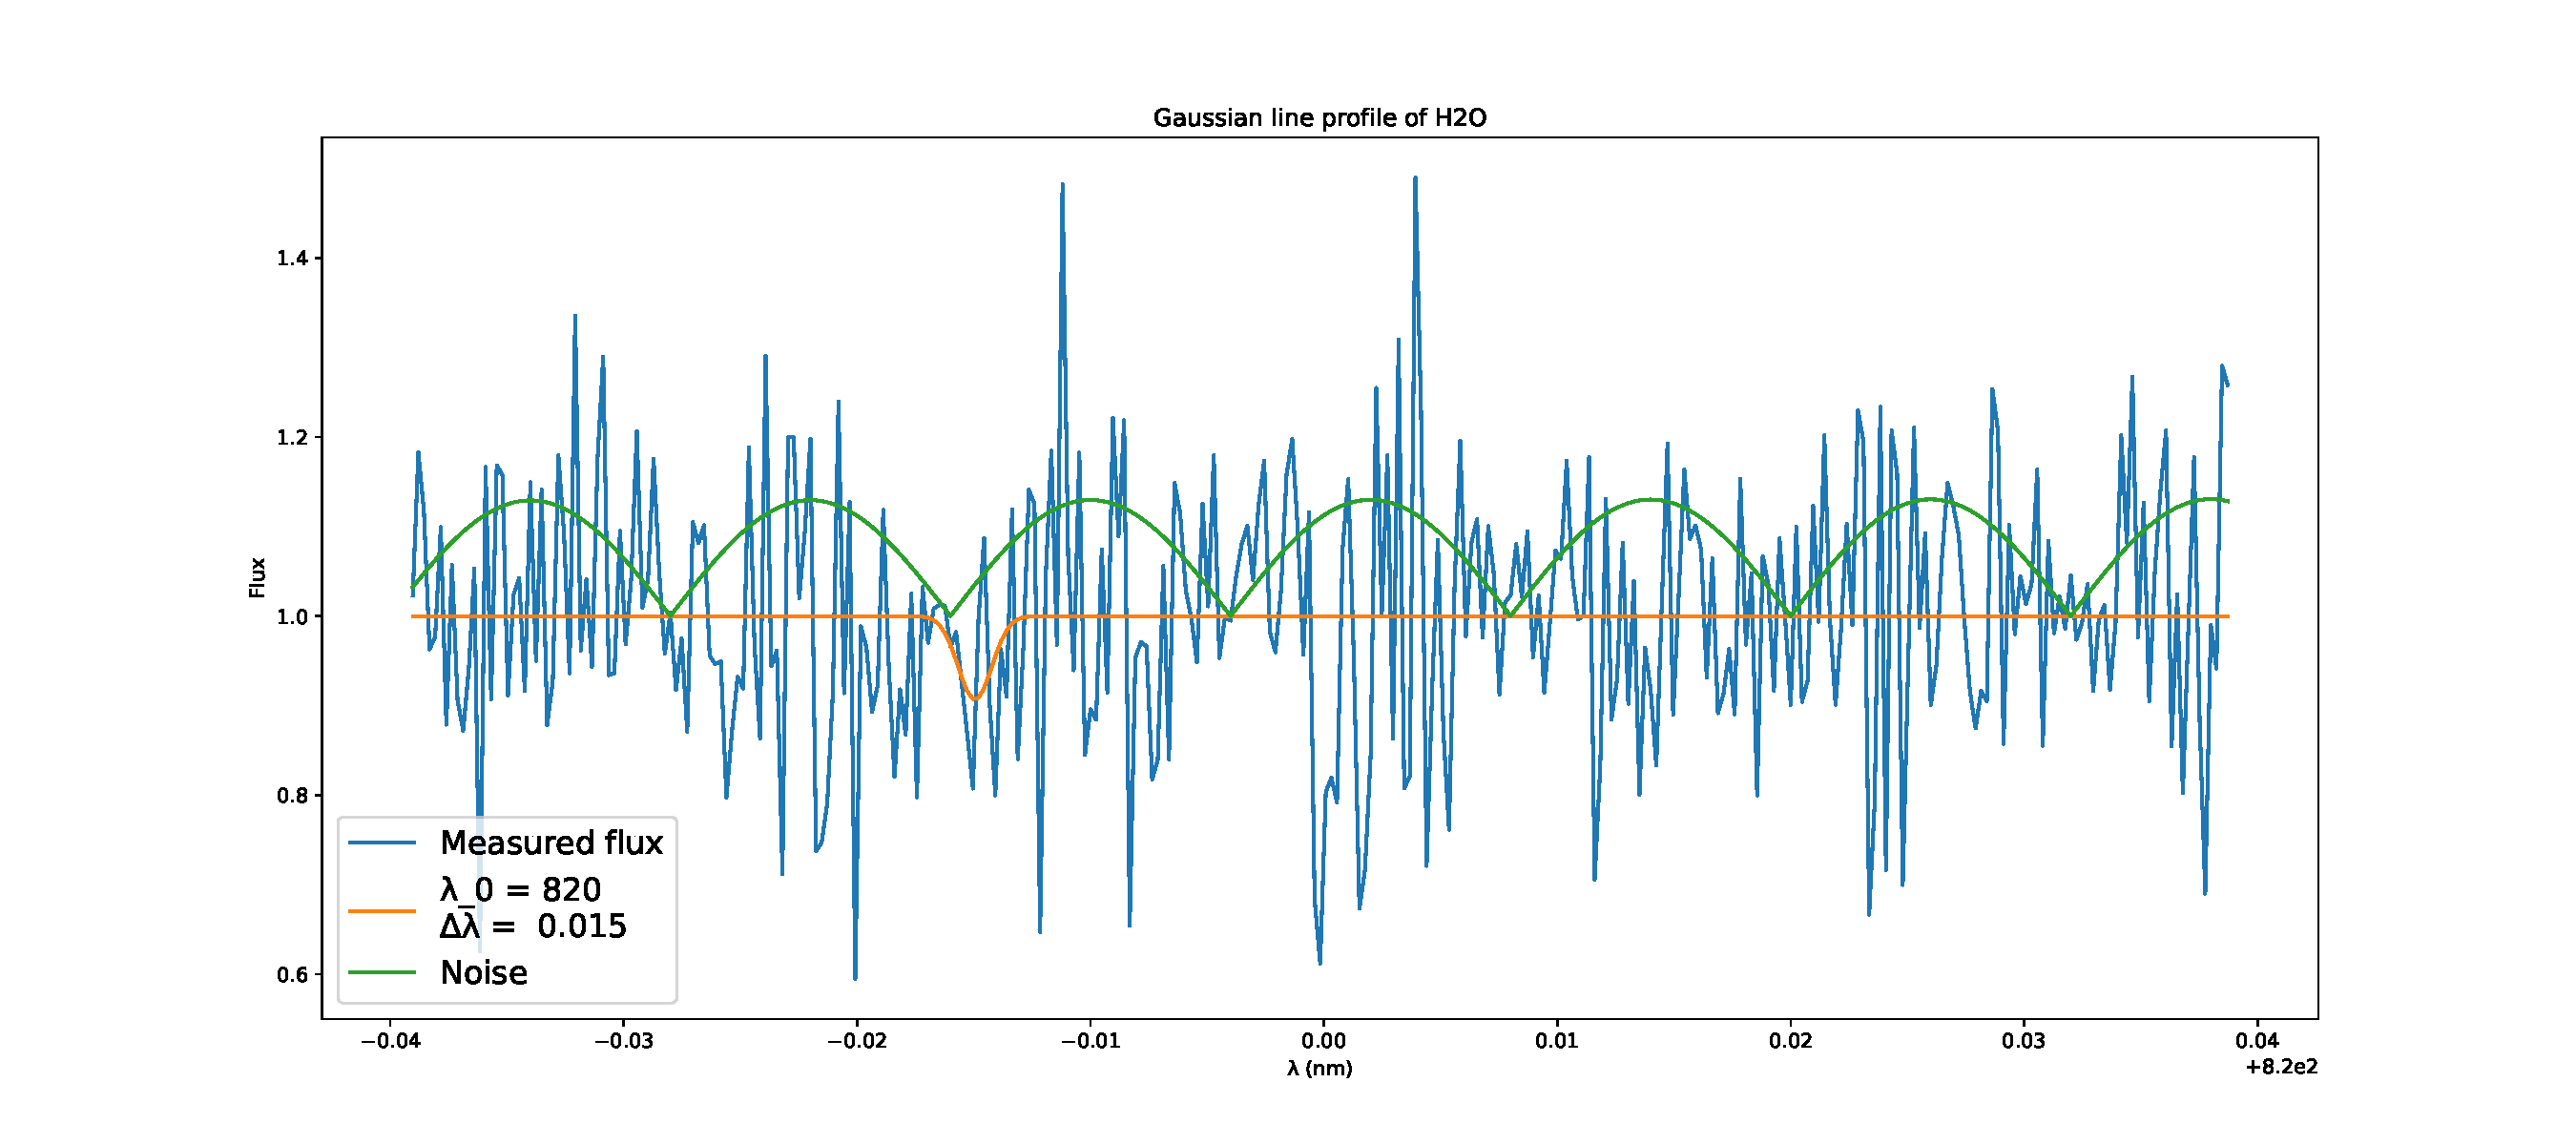
\includegraphics[scale =.3]{Figures/H2O 820}
      \caption{Flux Data and Spectral Line Analysis}
      \label{fig: H2 820}
    \end{figure}

    \begin{figure}[h!]
      \centering
      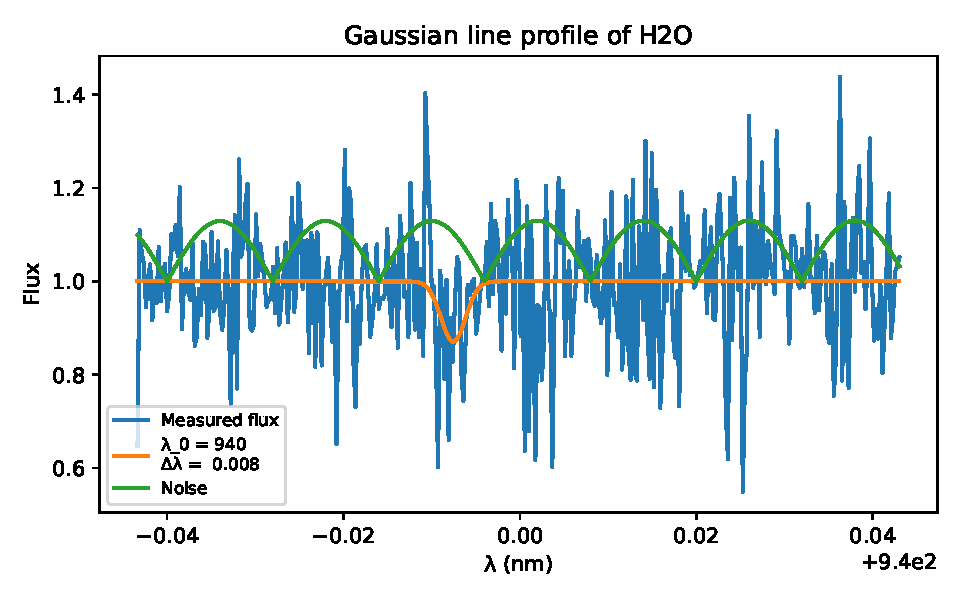
\includegraphics[scale =.3]{Figures/H2O 940}
      \caption{Flux Data and Spectral Line Analysis}
      \label{fig: H2 940}
    \end{figure}

    \begin{figure}[h!]
      \centering
      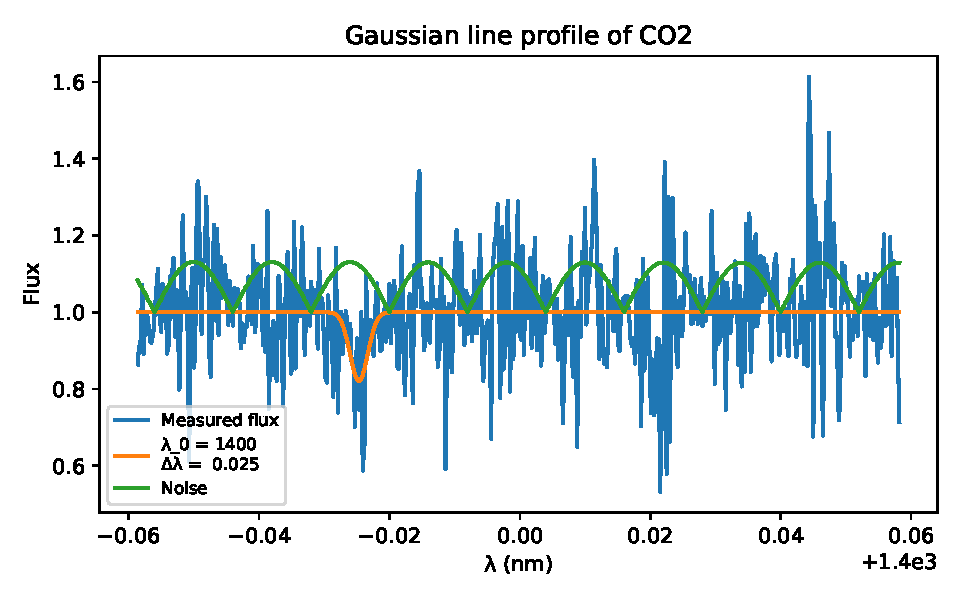
\includegraphics[scale =.3]{Figures/CO2 1400}
      \caption{Flux Data and Spectral Line Analysis}
      \label{fig: CO2 1400}
    \end{figure}

    \begin{figure}[h!]
      \centering
      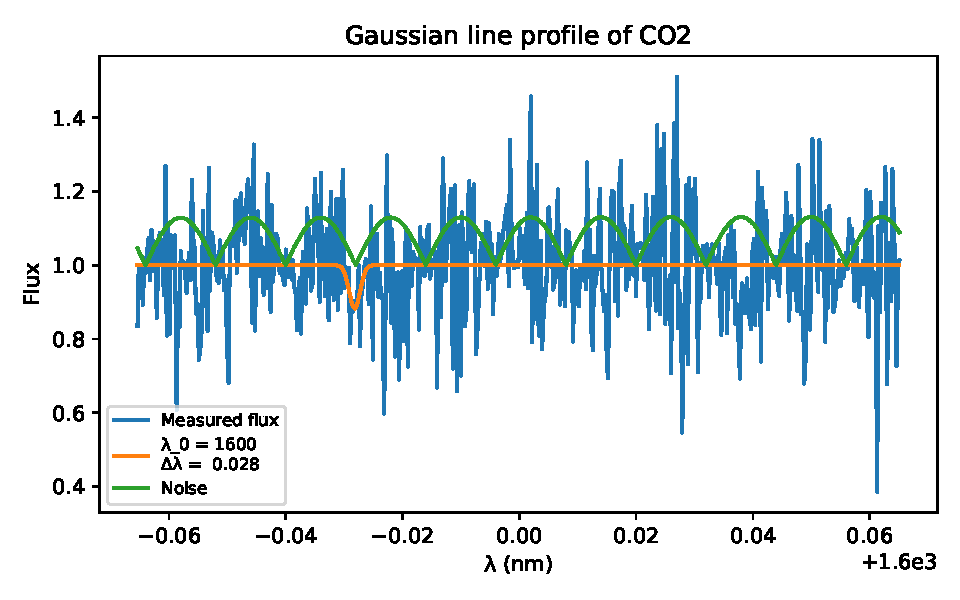
\includegraphics[scale =.3]{Figures/CO2 1600}
      \caption{Flux Data and Spectral Line Analysis}
      \label{fig: CO2 1600}
    \end{figure}

    \begin{figure}[h!]
      \centering
      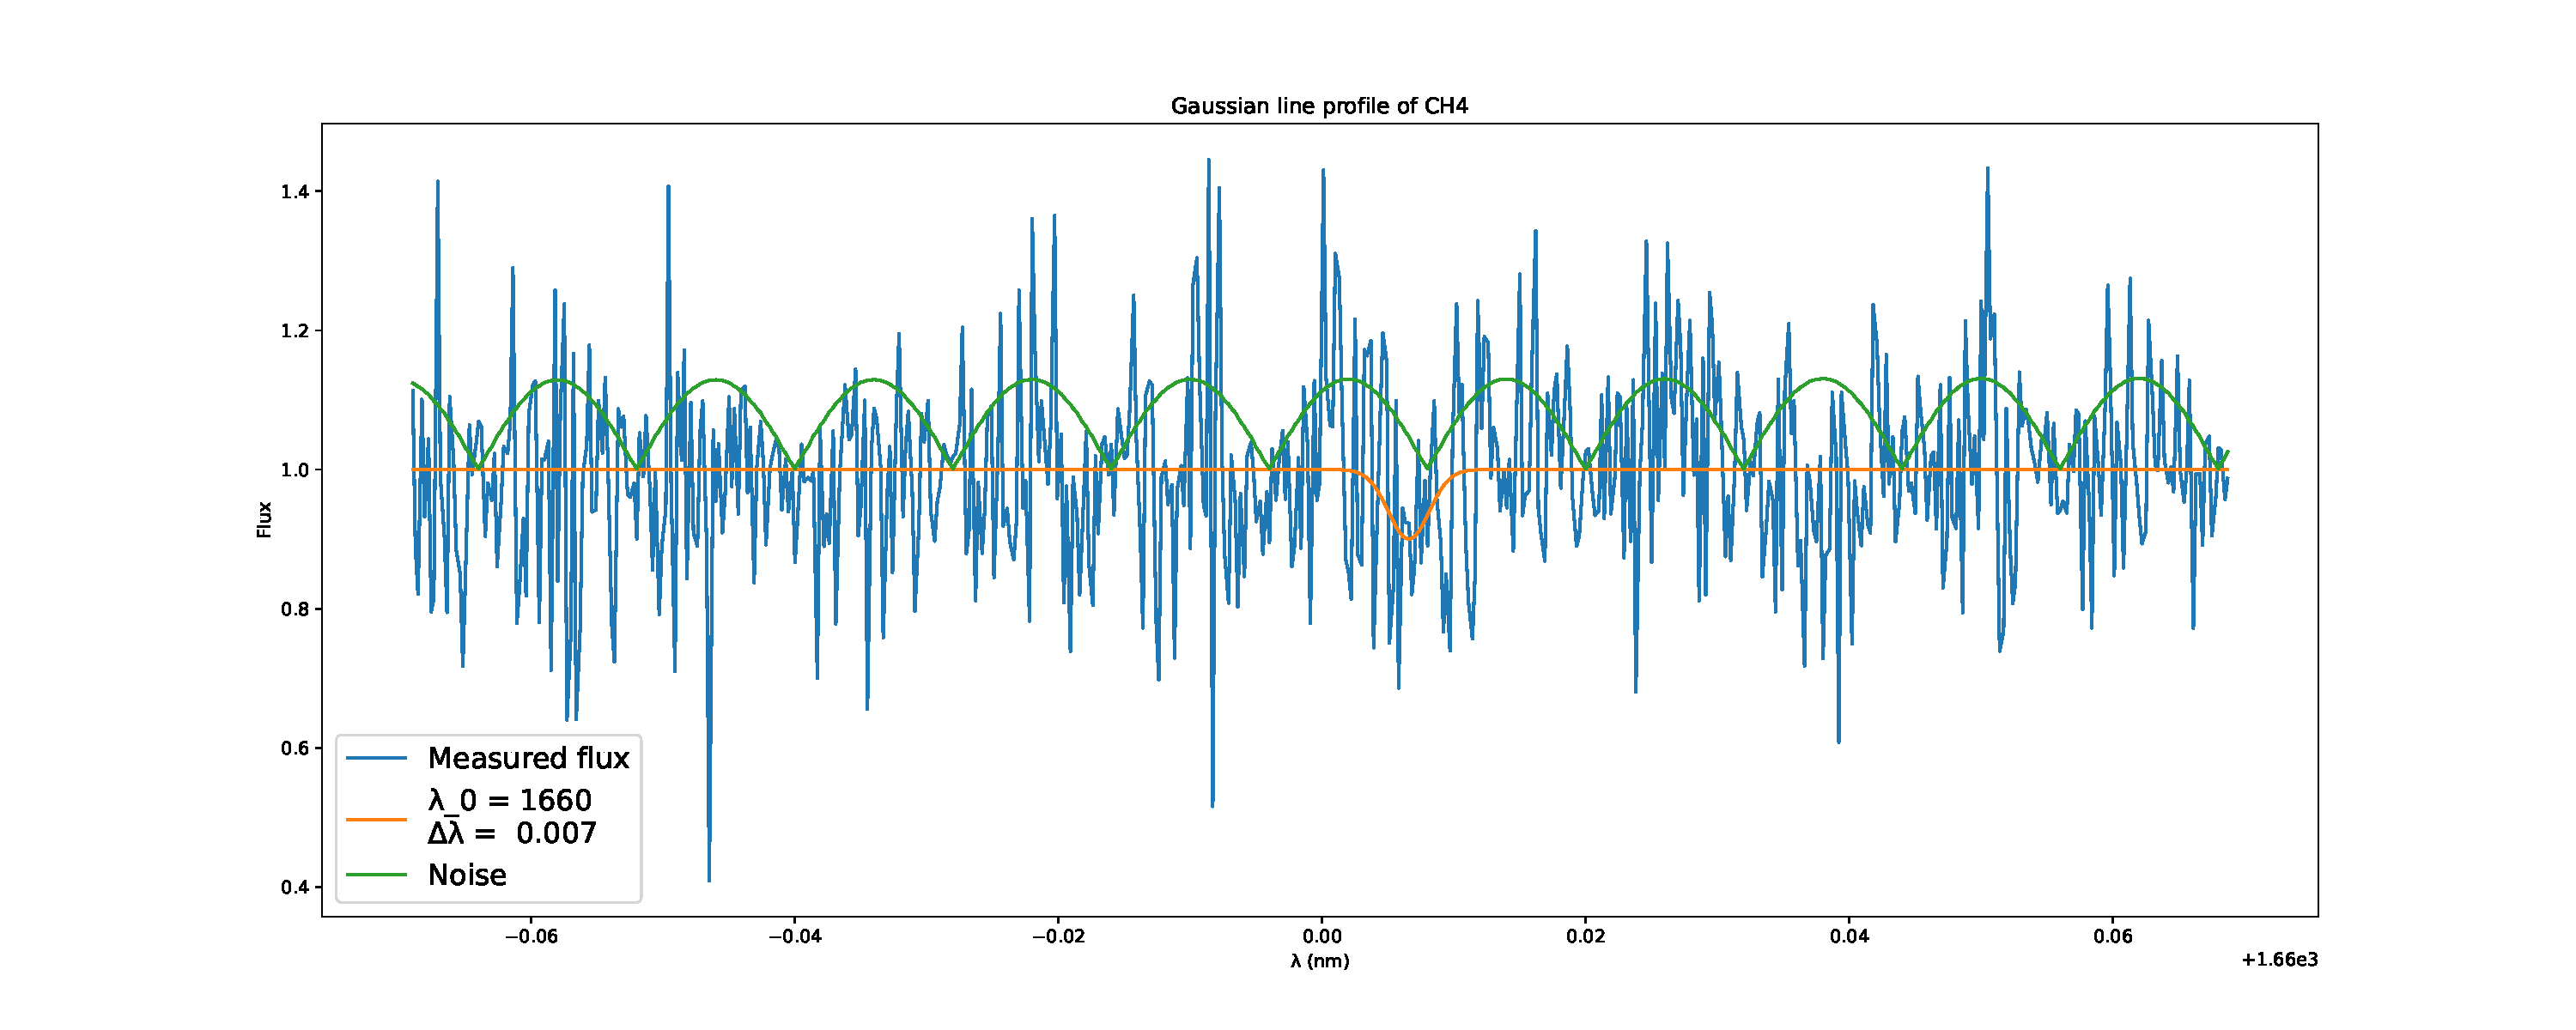
\includegraphics[scale =.3]{Figures/CH4 1660}
      \caption{Flux Data and Spectral Line Analysis}
      \label{fig: CH4 1660}
    \end{figure}

    \begin{figure}[h!]
      \centering
      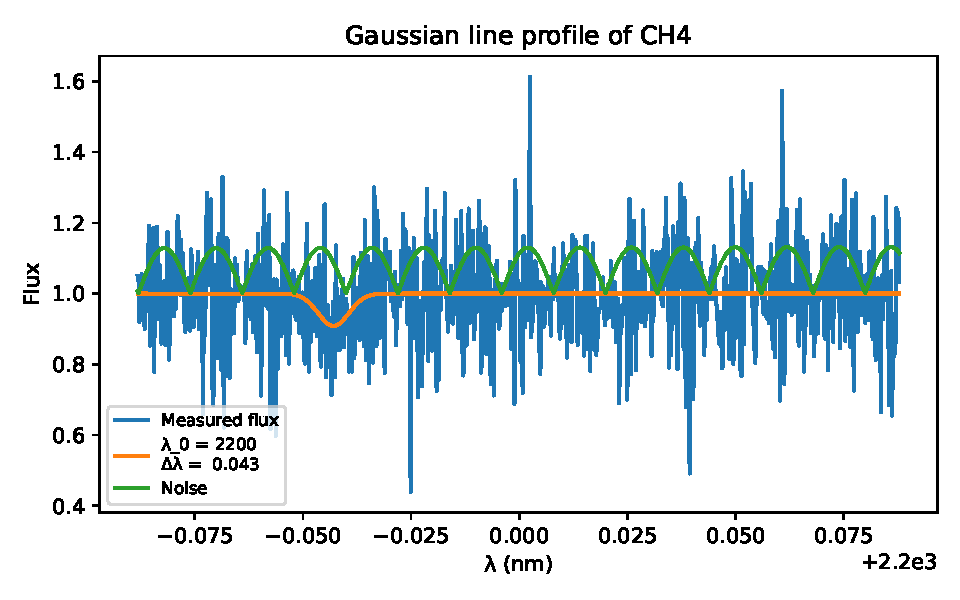
\includegraphics[scale =.3]{Figures/CH4 2200}
      \caption{Flux Data and Spectral Line Analysis}
      \label{fig: CH4 2200}
    \end{figure}

    \begin{figure}[h!]
      \centering
      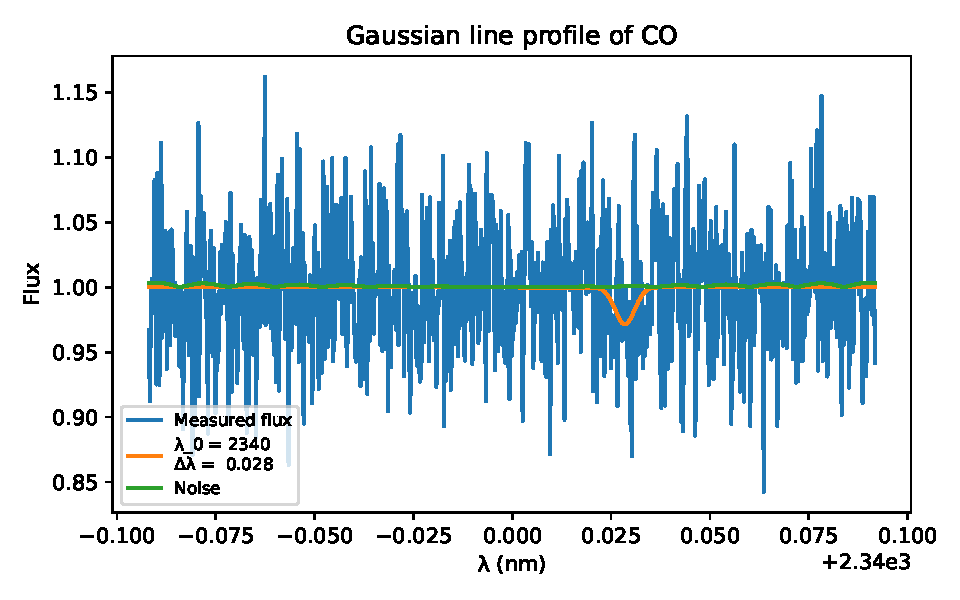
\includegraphics[scale =.3]{Figures/CO 2340}
      \caption{Flux Data and Spectral Line Analysis}
      \label{fig: CO 2340}
    \end{figure}

    \begin{figure}[h!]
      \centering
      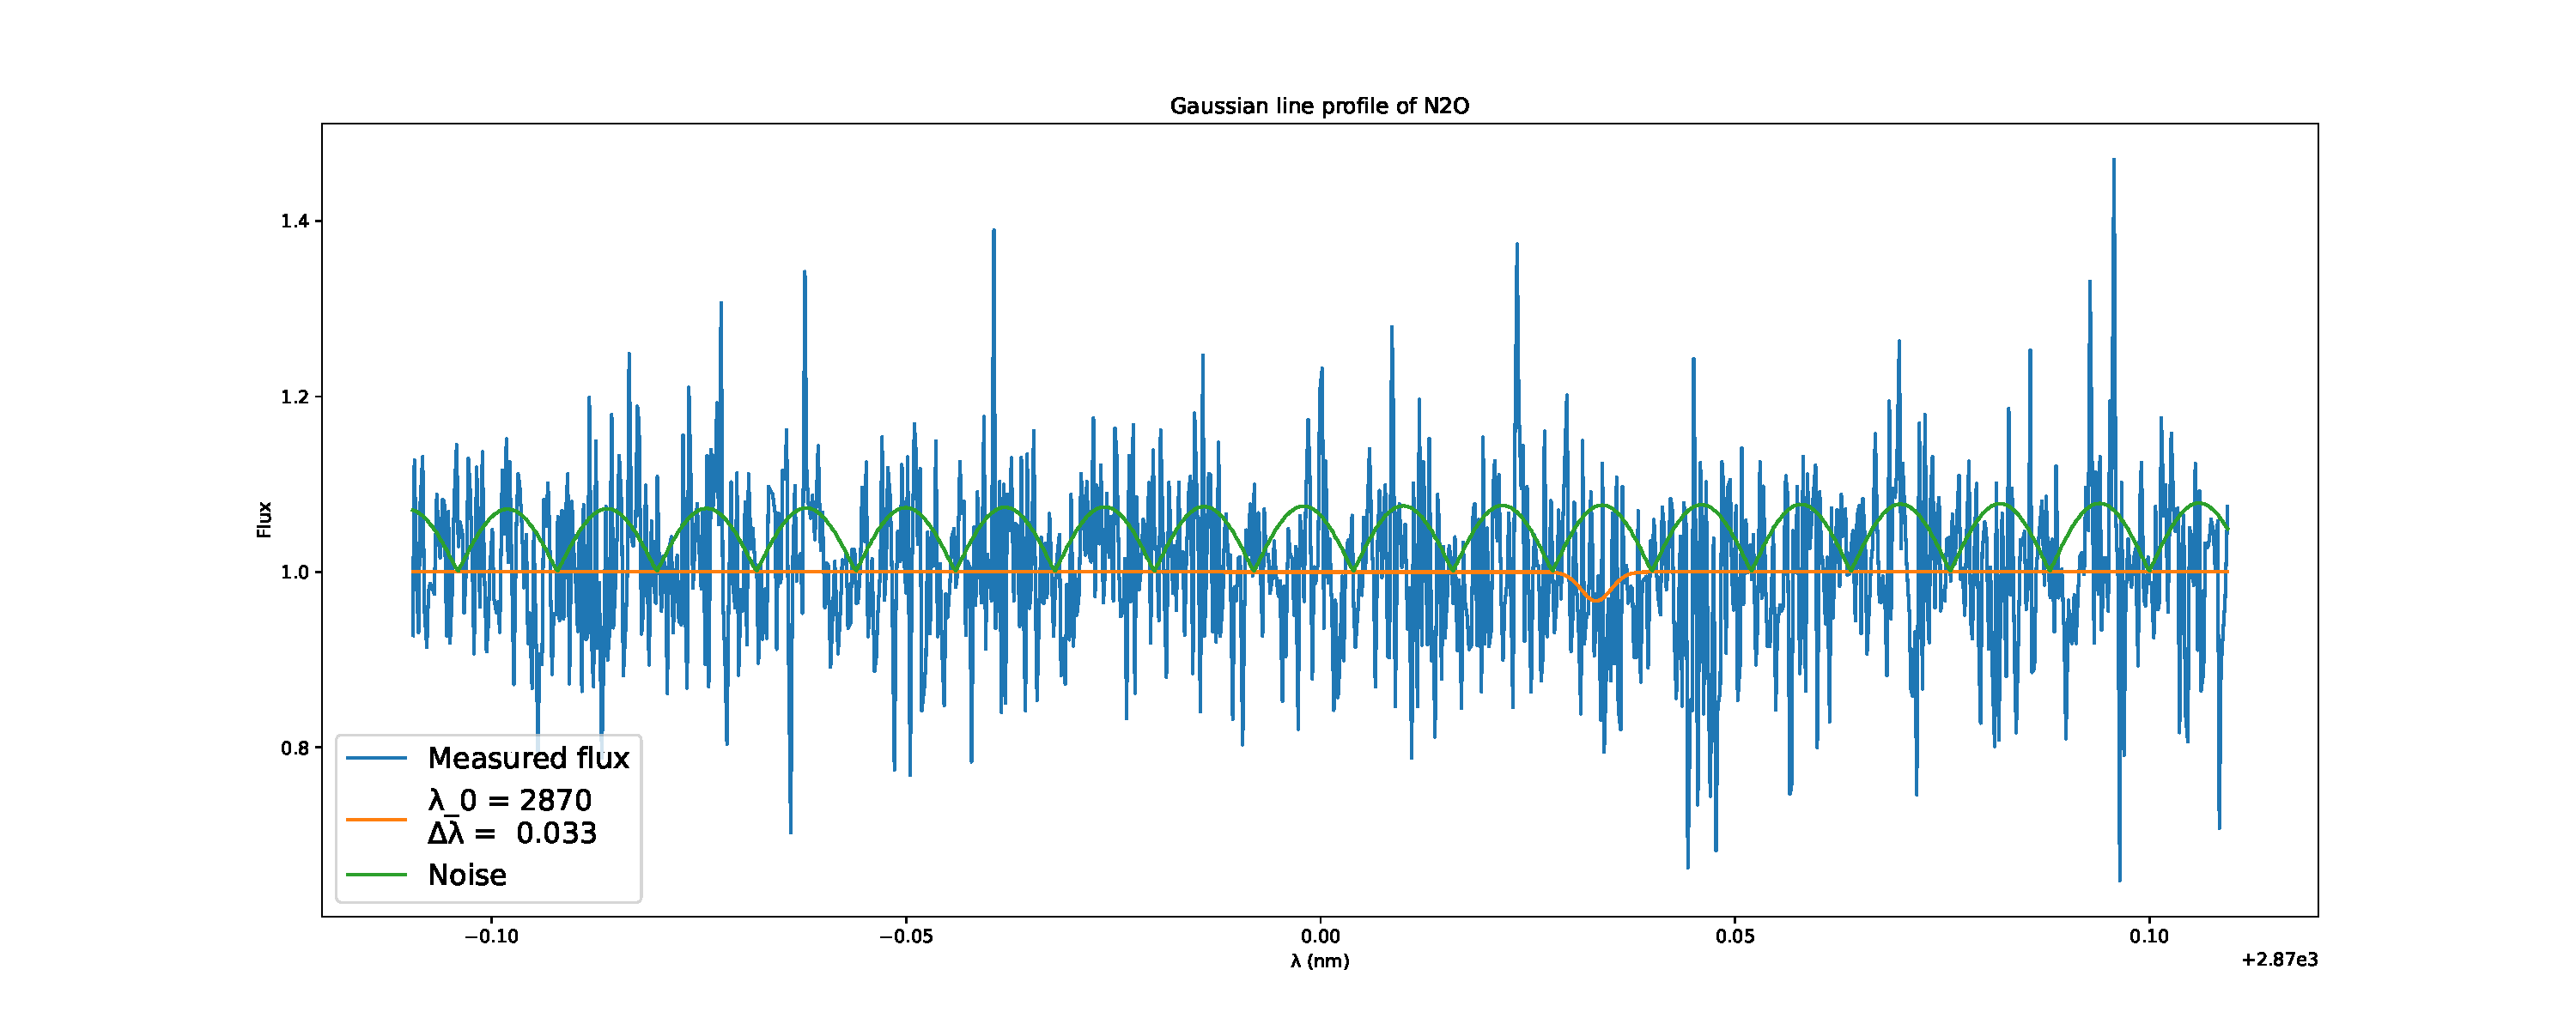
\includegraphics[scale =.3]{Figures/N2O 2870}
      \caption{Flux Data and Spectral Line Analysis}
      \label{fig: N20 2870}
    \end{figure}
\clearpage
\twocolumngrid

\subsection{Potential Landing sites}\label{subsec:potential-landing-sites}
    \begin{figure}[h]
        %% H(Here), h(here approx), t(top of page), b(bottom of page)
        \centering
        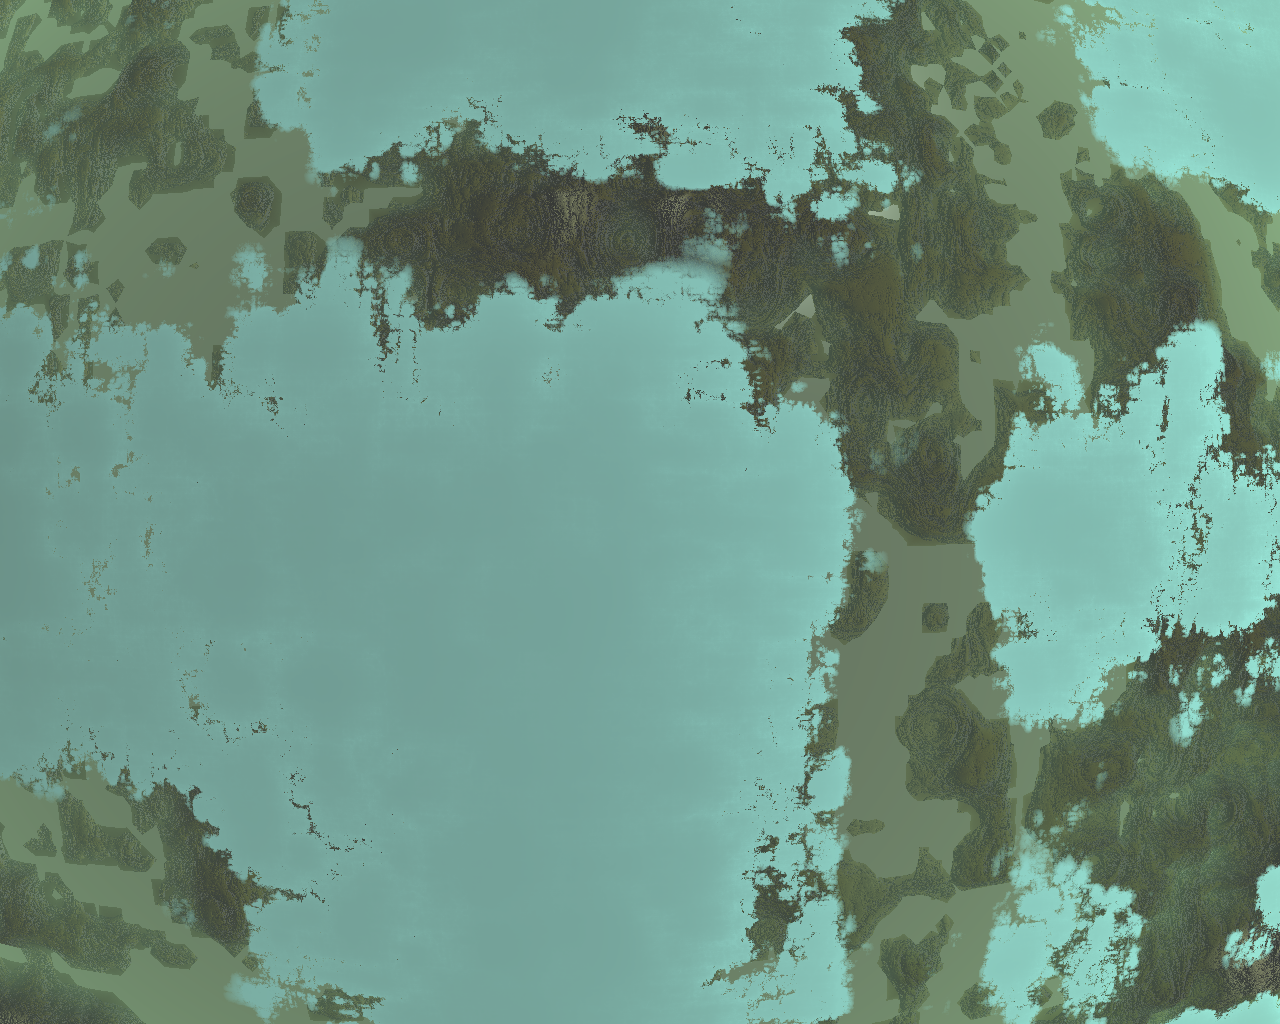
\includegraphics[scale=0.14]{Figures/l_site0}
        \caption{Picture of possible landing site 0 from the low-altitude orbit.}\label{fig:l_site0}
    \end{figure}
    \begin{figure}[h]
        %% H(Here), h(here approx), t(top of page), b(bottom of page)
        \centering
        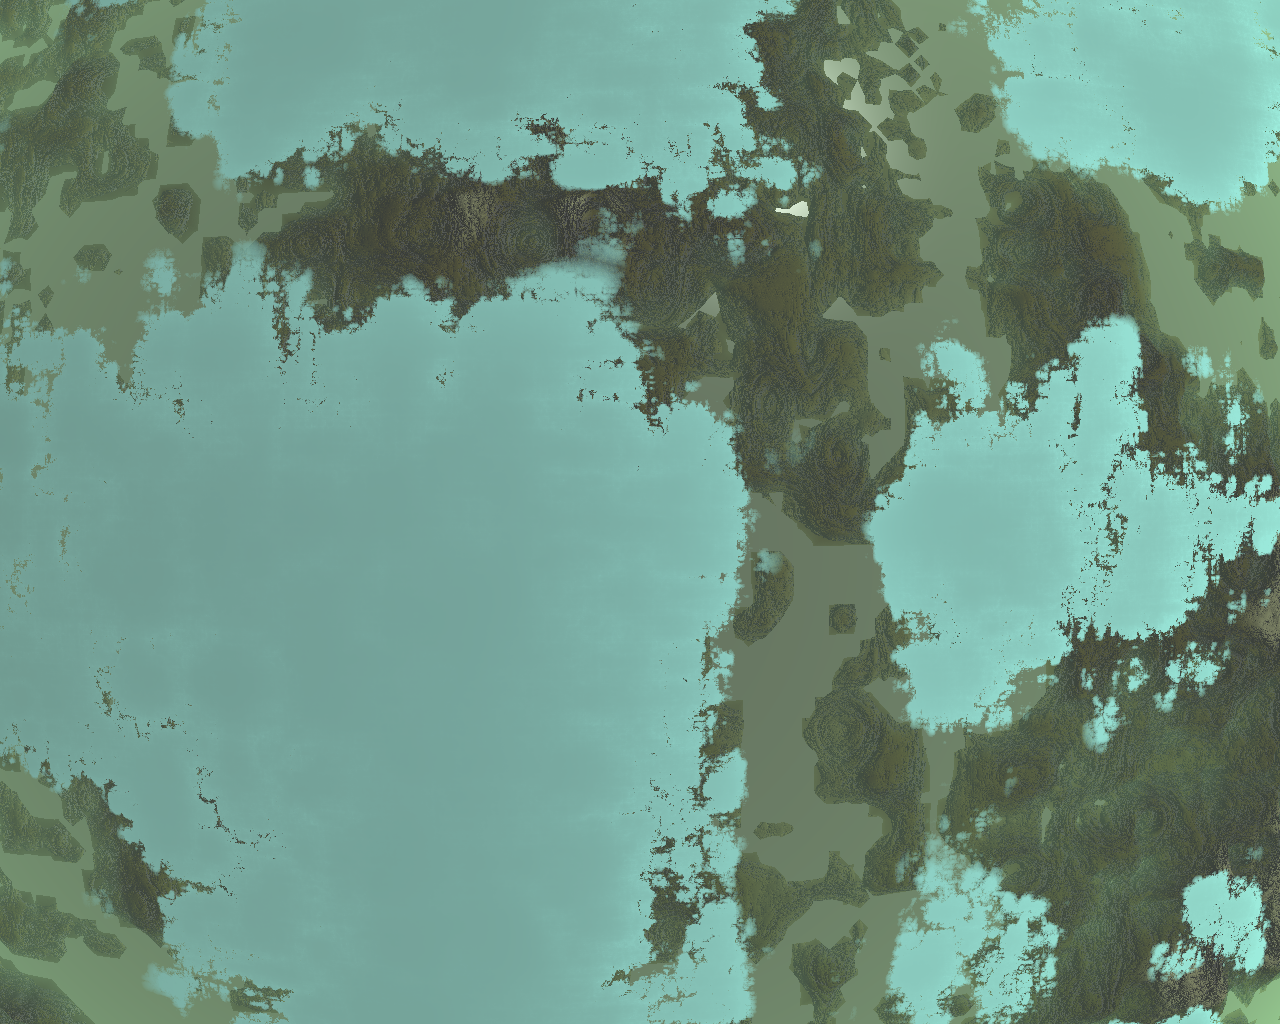
\includegraphics[scale=0.14]{Figures/l_site1}
        \caption{Picture of possible landing site 1 from the low-altitude orbit.}\label{fig:l_site1}
    \end{figure}
    \begin{figure}[h]
        %% H(Here), h(here approx), t(top of page), b(bottom of page)
        \centering
        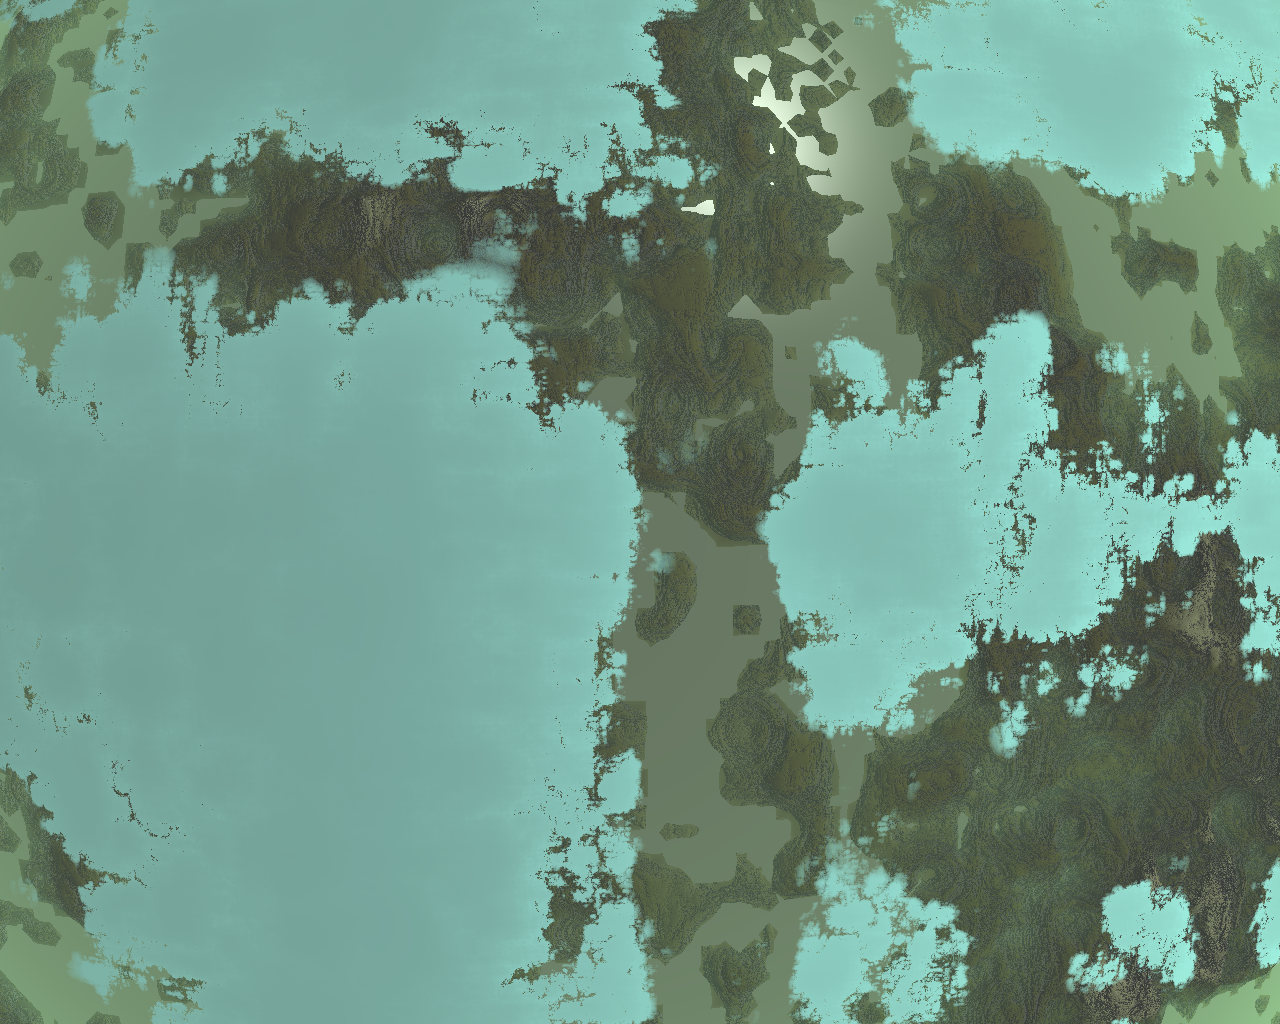
\includegraphics[scale=0.14]{Figures/l_site2}
        \caption{Picture of possible landing site 2 from the low-altitude orbit.}\label{fig:l_site2}
    \end{figure}
    \begin{figure}[h]
        %% H(Here), h(here approx), t(top of page), b(bottom of page)
        \centering
        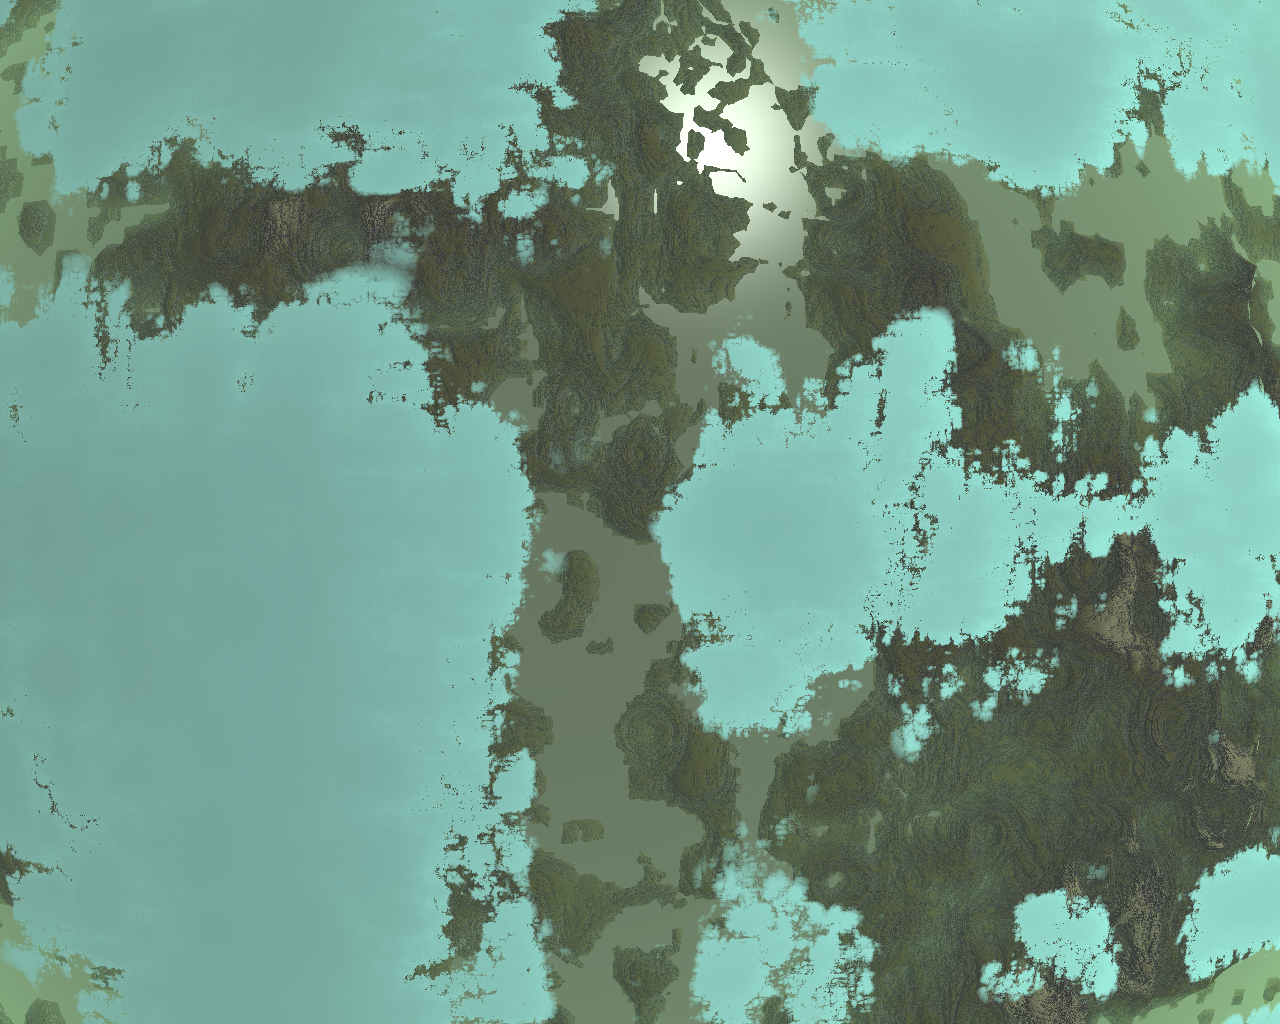
\includegraphics[scale=0.14]{Figures/l_site3}
        \caption{Picture of possible landing site 3 from the low-altitude orbit.}\label{fig:l_site3}
    \end{figure}
    \begin{figure}[h]
        %% H(Here), h(here approx), t(top of page), b(bottom of page)
        \centering
        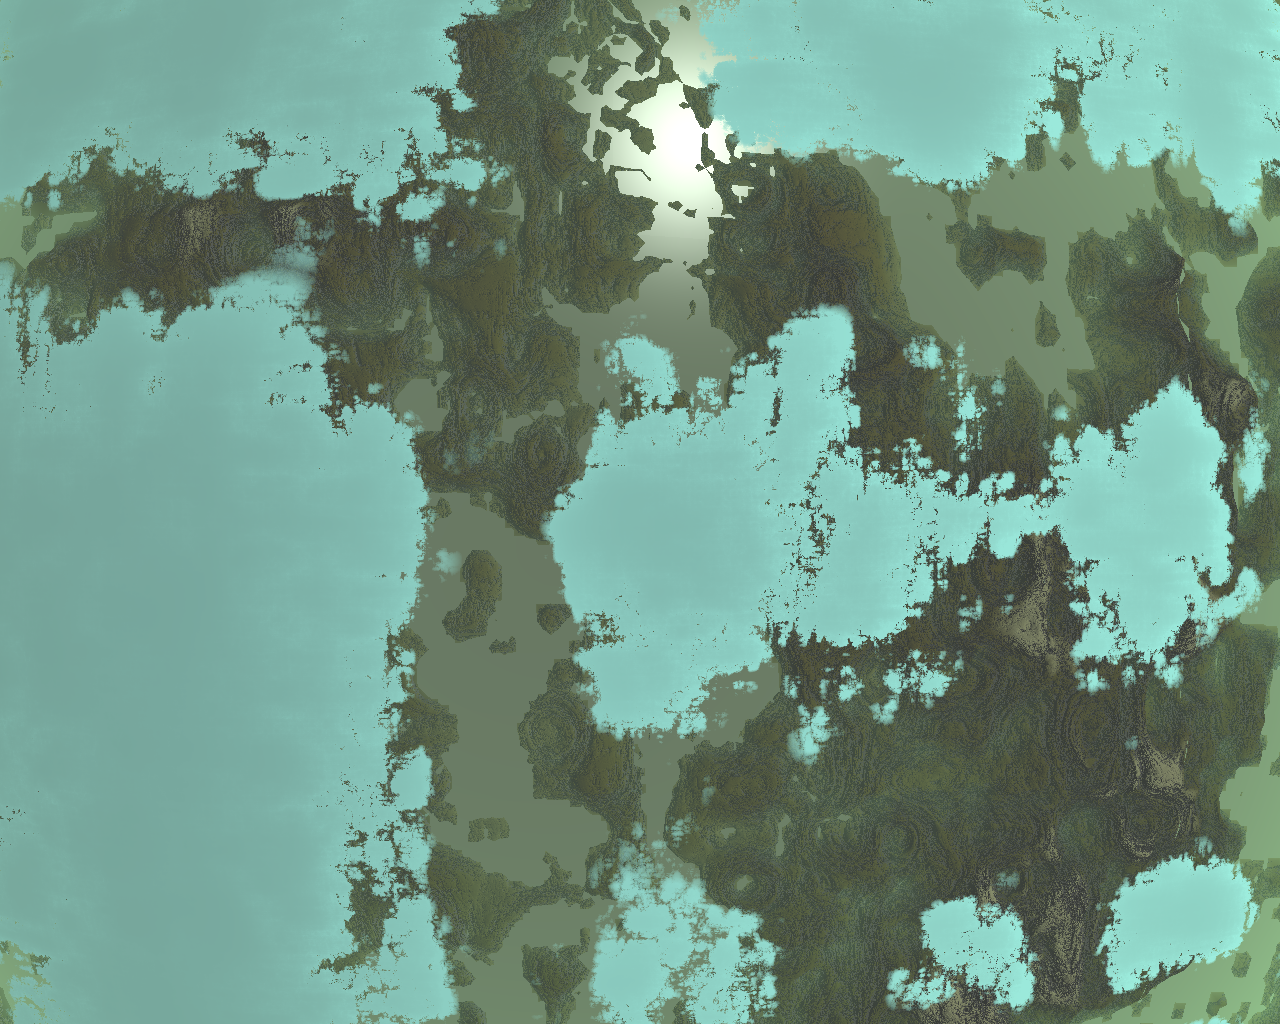
\includegraphics[scale=0.14]{Figures/l_site4}
        \caption{Picture of possible landing site 4 from the low-altitude orbit.}\label{fig:l_site4}
    \end{figure}
    \begin{figure}[h]
        %% H(Here), h(here approx), t(top of page), b(bottom of page)
        \centering
        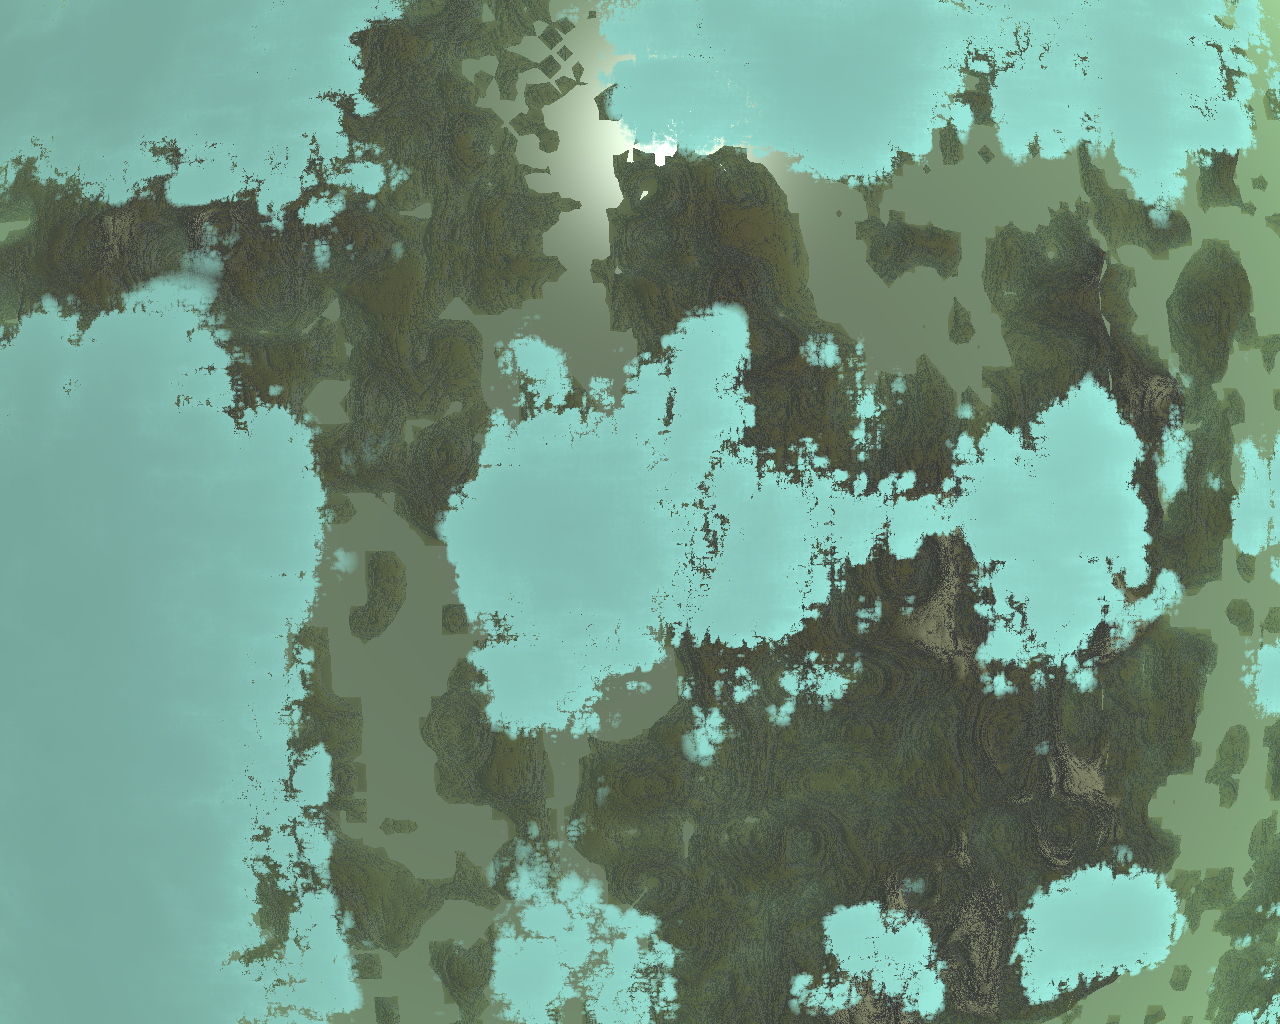
\includegraphics[scale=0.14]{Figures/l_site5}
        \caption{Picture of possible landing site 5 from the low-altitude orbit.}\label{fig:l_site5}
    \end{figure}
    \begin{figure}[h]
        %% H(Here), h(here approx), t(top of page), b(bottom of page)
        \centering
        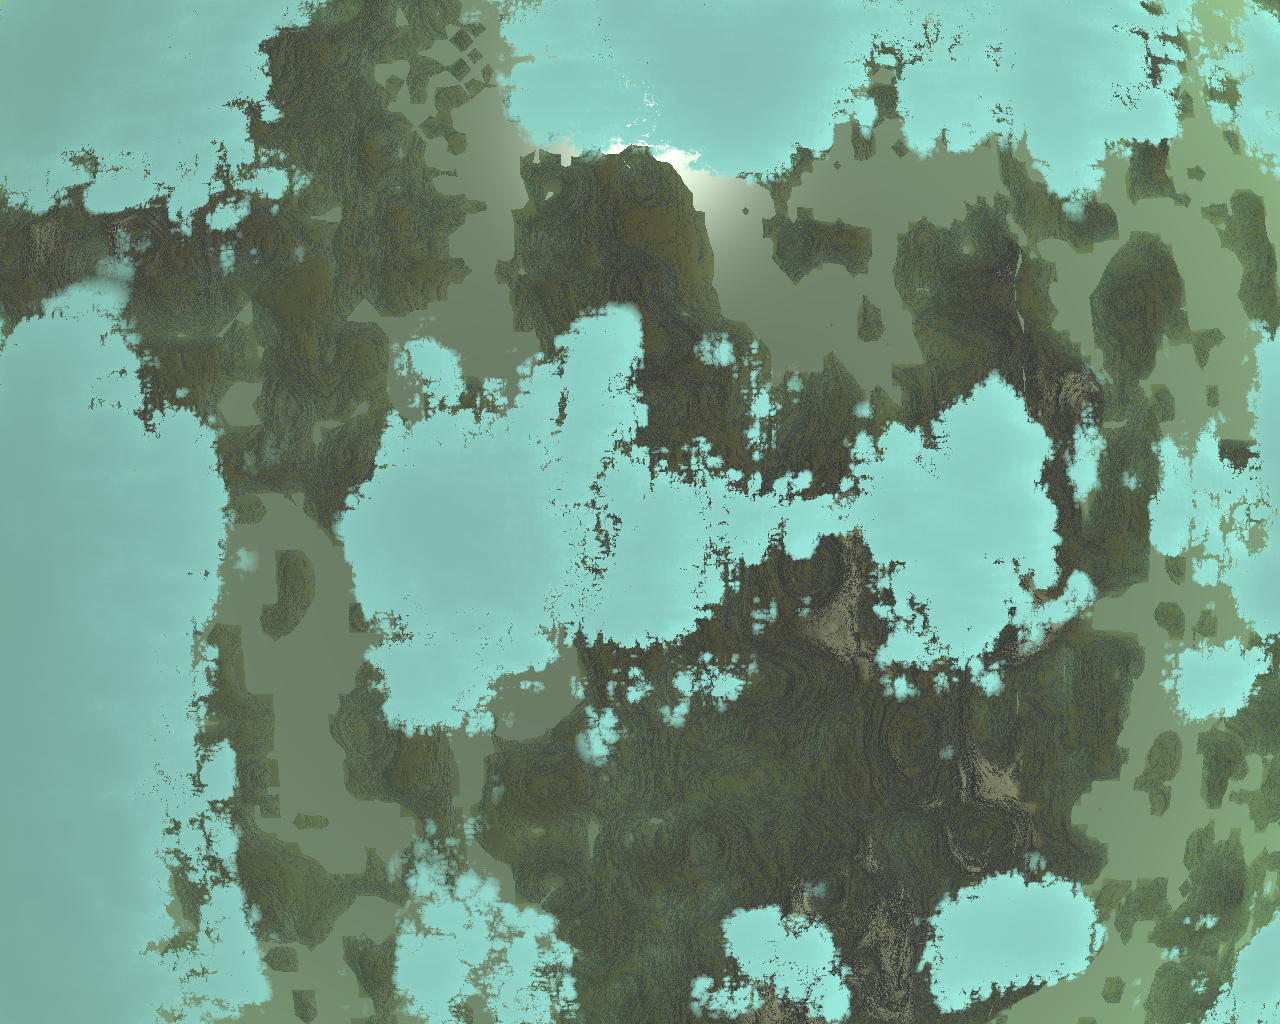
\includegraphics[scale=0.14]{Figures/l_site6}
        \caption{Picture of possible landing site 6 from the low-altitude orbit.}\label{fig:l_site6}
    \end{figure}
    \begin{figure}[h]
        %% H(Here), h(here approx), t(top of page), b(bottom of page)
        \centering
        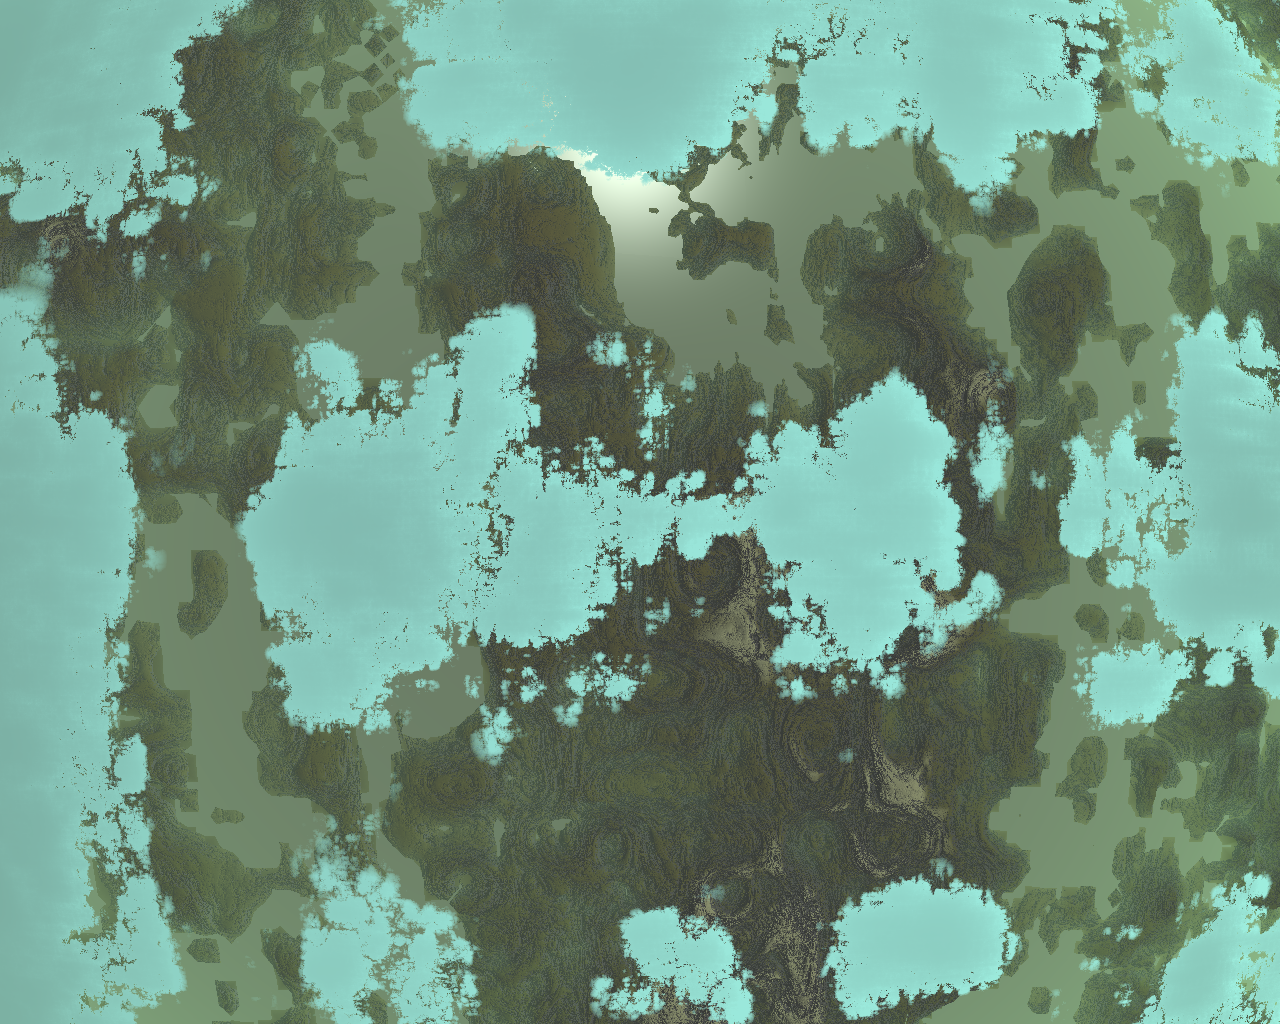
\includegraphics[scale=0.14]{Figures/l_site7}
        \caption{Picture of possible landing site 7 from the low-altitude orbit.}\label{fig:l_site7}
    \end{figure}
    \begin{figure}[h]
        %% H(Here), h(here approx), t(top of page), b(bottom of page)
        \centering
        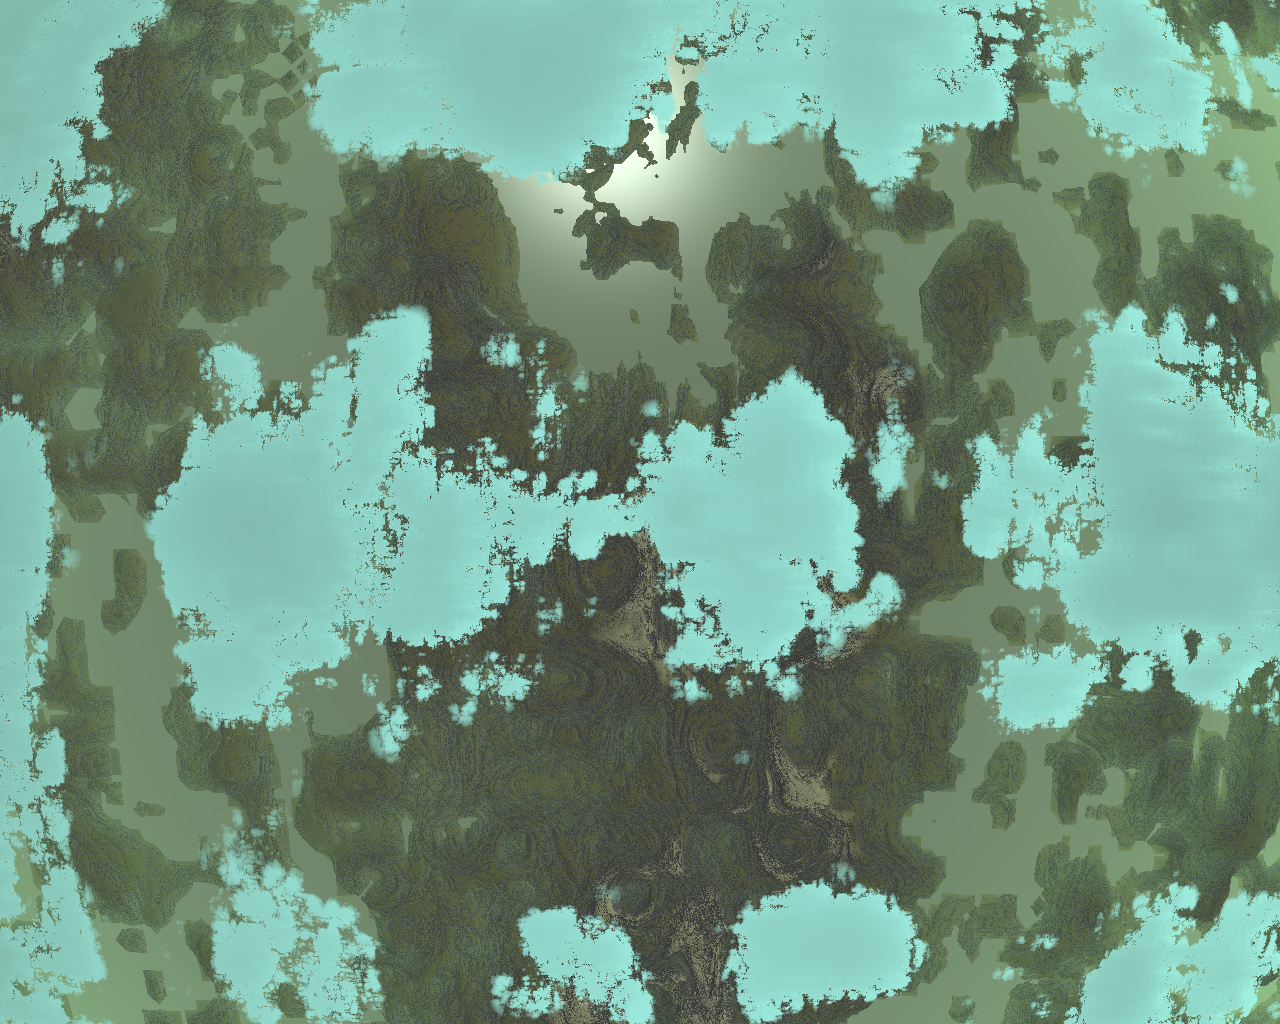
\includegraphics[scale=0.14]{Figures/l_site8}
        \caption{Picture of possible landing site 8 from the low-altitude orbit.}\label{fig:l_site8}
    \end{figure}
    \begin{figure}[h]
        %% H(Here), h(here approx), t(top of page), b(bottom of page)
        \centering
        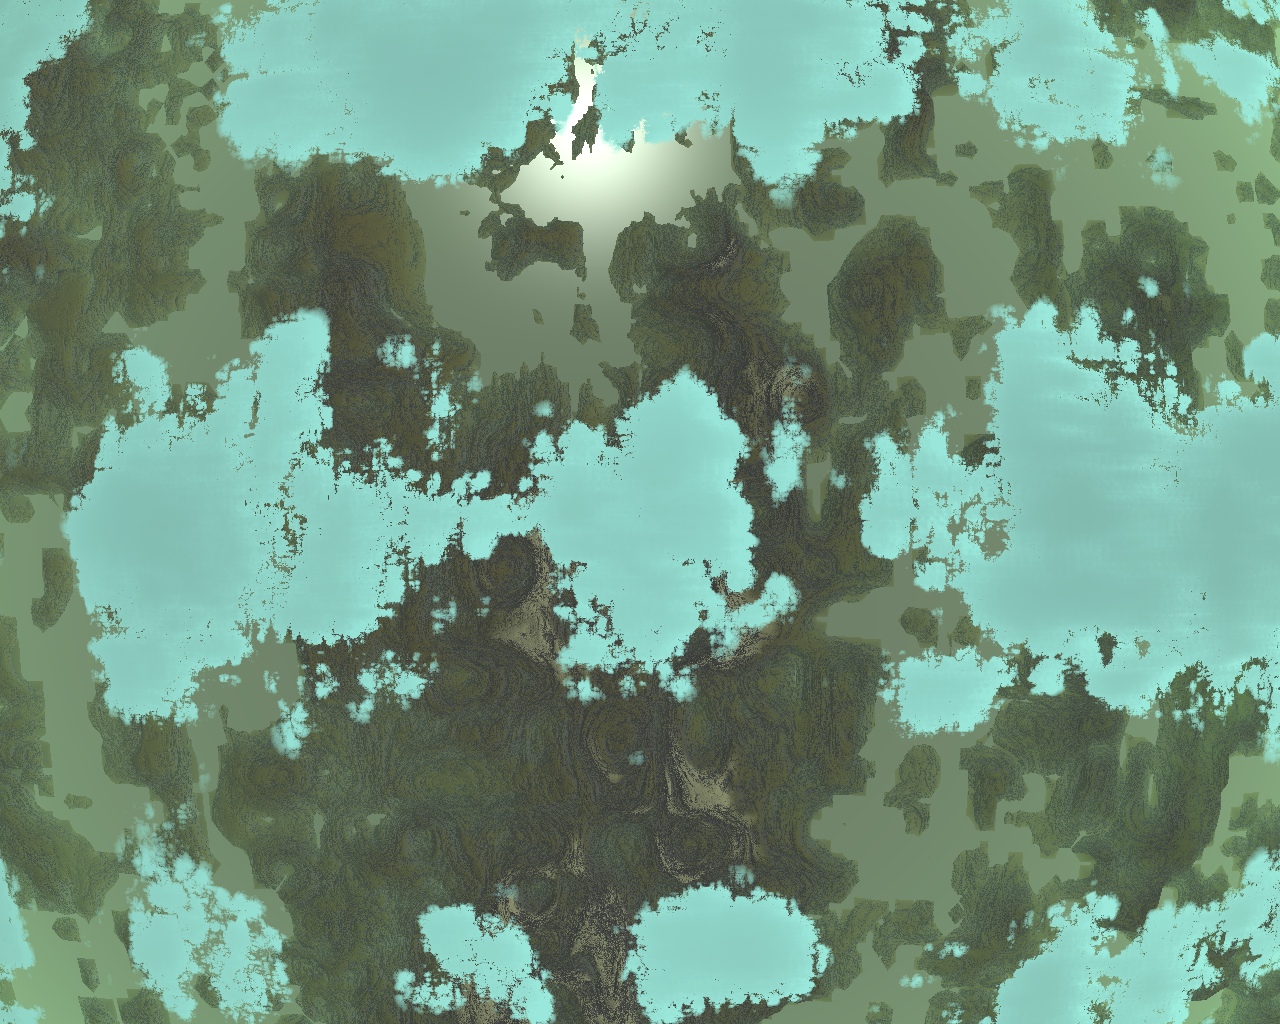
\includegraphics[scale=0.14]{Figures/l_site9}
        \caption{Picture of possible landing site 9 from the low-altitude orbit.}\label{fig:l_site9}
    \end{figure}
    \begin{figure}[h]
        %% H(Here), h(here approx), t(top of page), b(bottom of page)
        \centering
        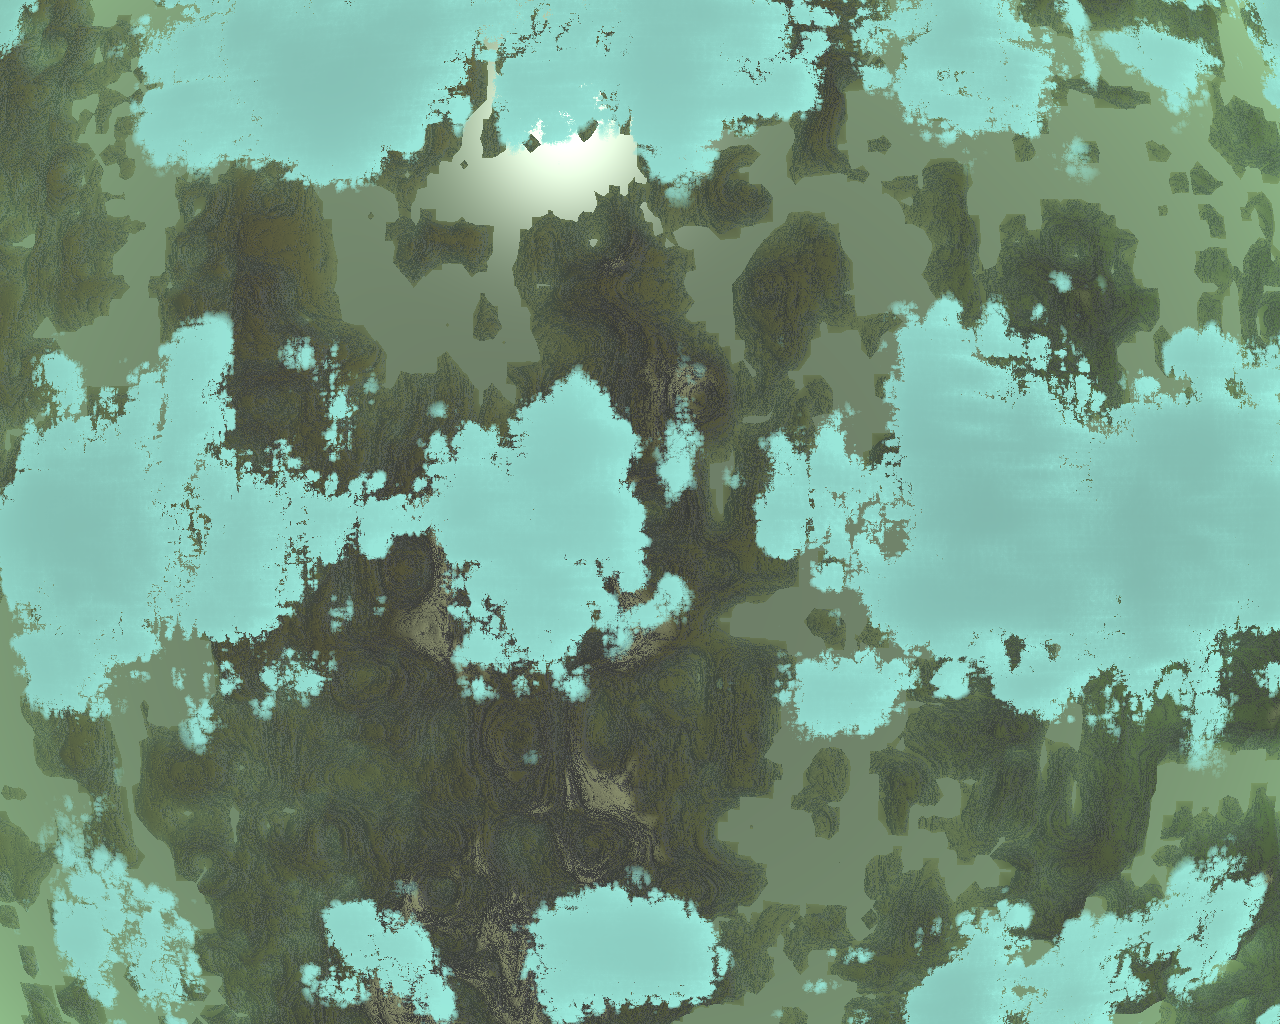
\includegraphics[scale=0.14]{Figures/l_site10}
        \caption{Picture of possible landing site 10 from the low-altitude orbit.}\label{fig:l_site10}
    \end{figure}
    \begin{figure}[h]
        %% H(Here), h(here approx), t(top of page), b(bottom of page)
        \centering
        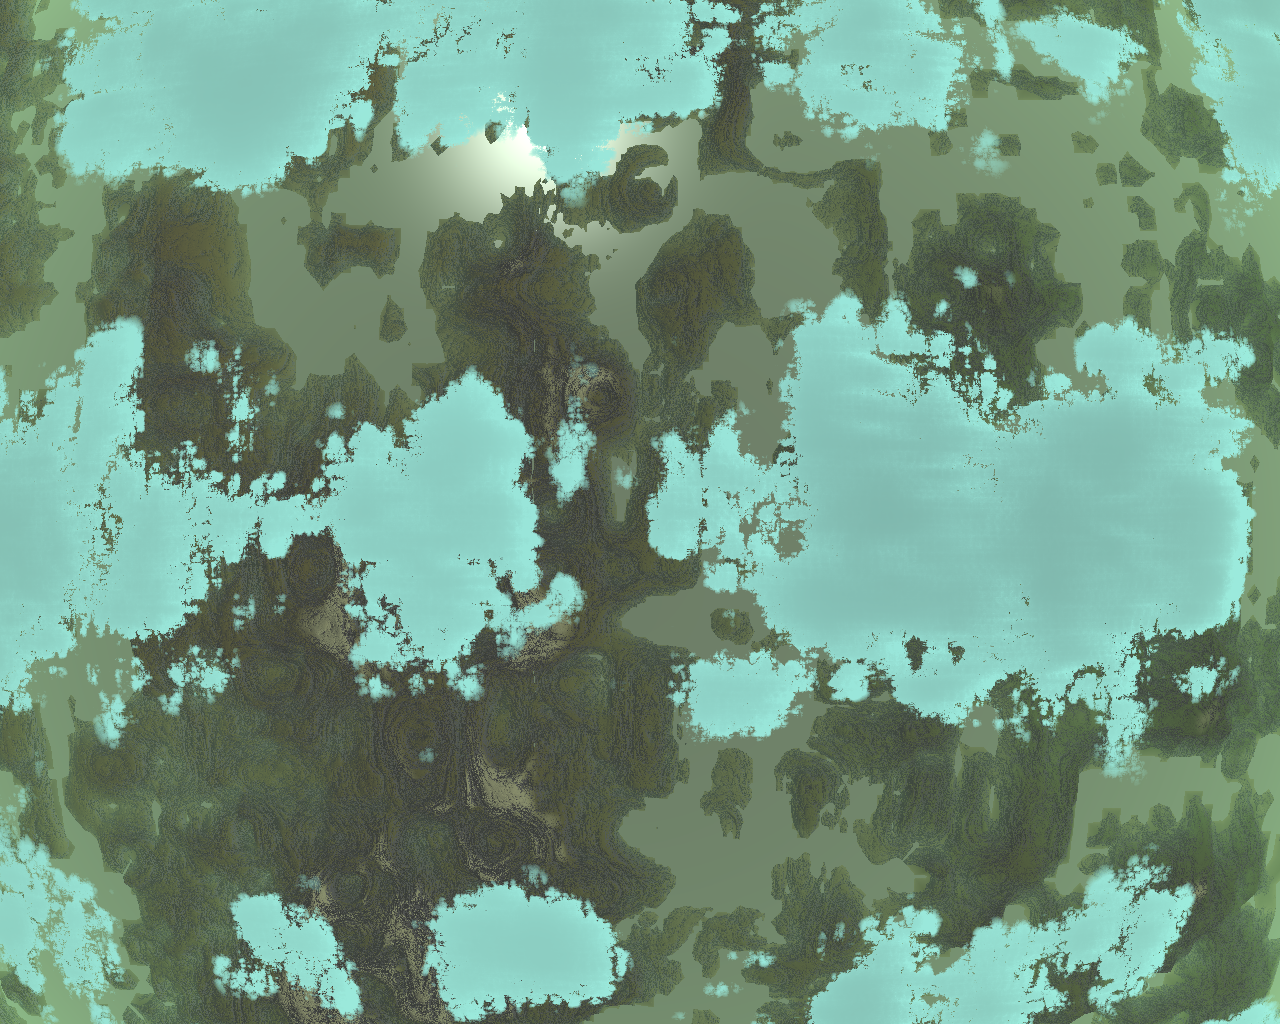
\includegraphics[scale=0.14]{Figures/l_site11}
        \caption{Picture of possible landing site 11 from the low-altitude orbit.}\label{fig:l_site11}
    \end{figure}
    \begin{figure}[h]
        %% H(Here), h(here approx), t(top of page), b(bottom of page)
        \centering
        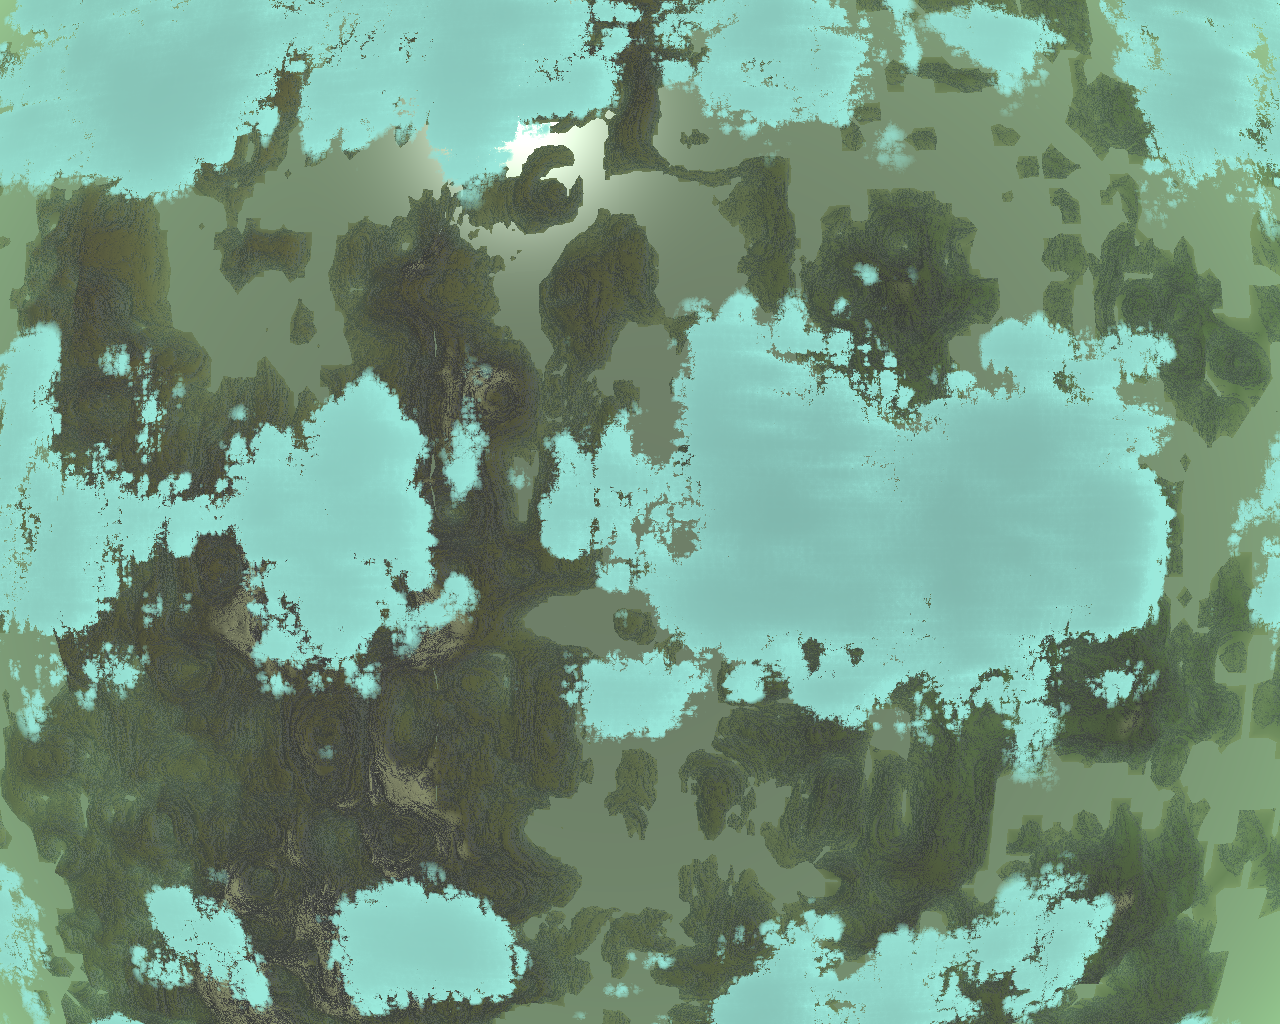
\includegraphics[scale=0.14]{Figures/l_site12}
        \caption{Picture of possible landing site 12 from the low-altitude orbit.}\label{fig:l_site12}
    \end{figure}
    \begin{figure}[h]
        %% H(Here), h(here approx), t(top of page), b(bottom of page)
        \centering
        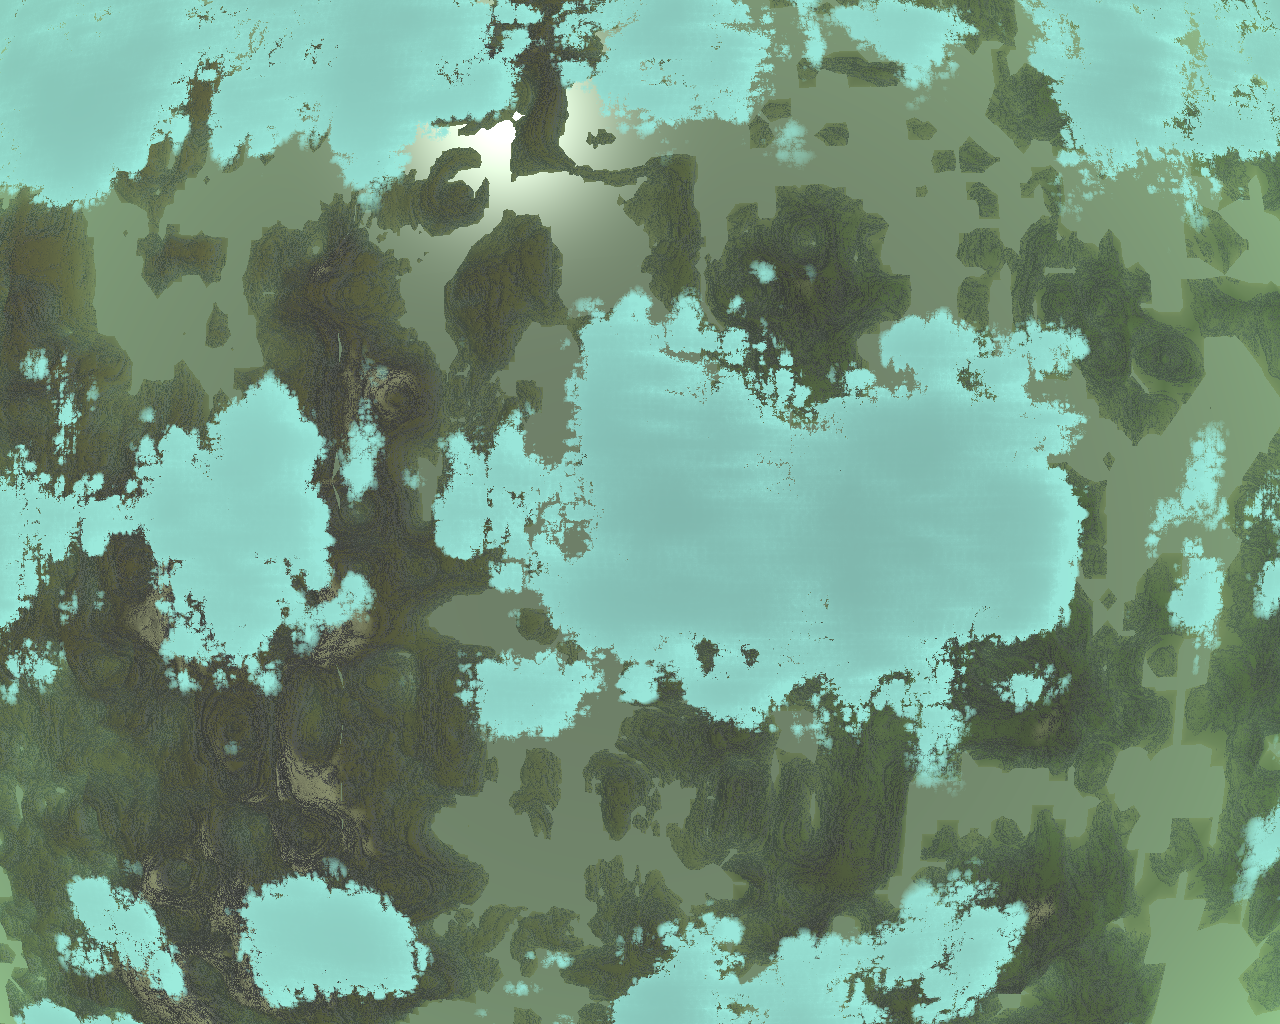
\includegraphics[scale=0.14]{Figures/l_site13}
        \caption{Picture of possible landing site 13 from the low-altitude orbit.}\label{fig:l_site13}
    \end{figure}
    \begin{figure}[h]
        %% H(Here), h(here approx), t(top of page), b(bottom of page)
        \centering
        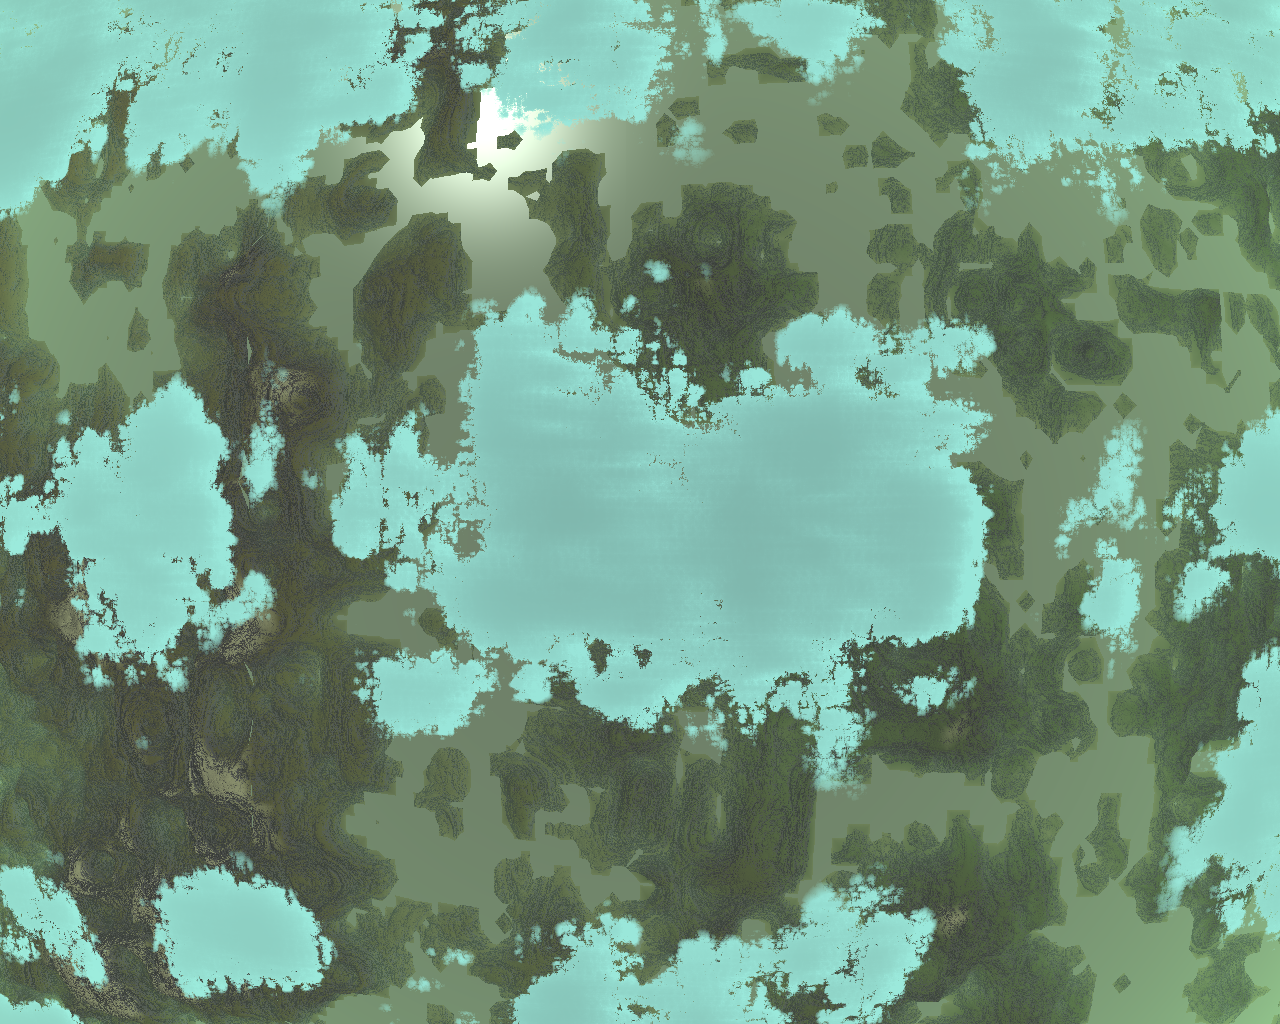
\includegraphics[scale=0.14]{Figures/l_site14}
        \caption{Picture of possible landing site 14 from the low-altitude orbit.}\label{fig:l_site14}
    \end{figure}

\section*{References} \label{sec: references}

\end{document}

